\documentclass[../main.tex]{subfiles}
\usepackage{slashed}
\usepackage[table]{xcolor}
\usepackage{hhline}
\usepackage{lipsum}

\let\Bbbk\relax
\usepackage{amsmath}
\usepackage{amsfonts}
\usepackage{simpler-wick}

\begin{document}
\setchapterimage[6.5cm]{images_ch6/wormhole.jpeg}
\setchapterpreamble[u]{\margintoc}
\chapter[Simmetrie Spazio-Temporali]{Simmetrie Spazio-Temporali}
% \labch{spacetime_symm}
\label{ch:spacetime_symm}
\fboxsep =1pt % separazione per i box


\section{Introduzione}
Consideriamo una prospettiva differente dal solito, ponendo in primo piano il ruolo delle particelle.

La situazione si presenta in questo modo: supponiamo di avere a che fare con uno stato iniziale multi-particellare $|\psi\rangle$, vogliamo calcolare la probabilità di transizione \(P\big(|\psi\rangle\rightarrow|\varphi\rangle\big)\) in presenza di una Hamiltoniana di interazione \( H_\text{int}\).

\[
|\psi\rangle \xrightarrow[]{ H_\text{int}} |\varphi\rangle \Rightarrow P\big(|\psi\rangle\rightarrow|\varphi\rangle\big) = | \langle\psi|\varphi\rangle |^2
\]

Il problema che ci si pone davanti è duplice:
\begin{enumerate}
    \item[\textbf{1)}] Vorremmo costruire in maniere esplicita lo stato $|\psi\rangle$ ed il suo spazio di Hilbert.
    
    \item[\textbf{2)}] Ci piacerebbe rendere il calcolo delle probabilità di transizione compatibile con il principio della relatività, i.e. \textit{“due osservatori inerziali che svolgono lo stesso esperimento quanto-meccanico devono ottenere lo stesso risultato.”}

    In un linguaggio più matematico, quello che vogliamo fare è \textbf{promuovere le trasformazioni del gruppo di Poincaré} (che in sostanza connettono diversi sistemi di riferimento inerziali per mezzo dei principi della relatività speciale) \textbf{a trasformazioni di simmetria per la meccanica quantistica}.
\end{enumerate}

\begin{definition}
    \textbf{(Trasformazione di Simmetria - v1.)}

    Si definisce TdS una trasformazione di stati sotto la quale le proprietà fisiche di un sistema quantistico non cambiano.
    \label{def:symmetry_transf_states}
\end{definition}

In particolare, siamo interessati alle trasformazioni di simmetria che lascino invariate le probabilità di transizione, ovvero tutte le possibili misure che possono essere fatte sul sistema quantistico in esame.

\subsection{Raggi e teorema di Wigner}
In meccanica quantistica, due vettori \(|\psi\rangle\) e \(\xi|\psi\rangle\) (con \(\xi \in \mathbb C,~ \xi\neq0\)) hanno esattamente lo stesso significato fisico.

Per questo motivo diciamo spesso che uno stato fisico non corrisponde ad un vettore nello spazio di Hilbert, bensì ad un raggio, i.e. un sottospazio 1-dimensionale definito da tutti i multipli complessi di un certo vettore.

Inoltre possiamo sempre scegliere \(c\) in modo tale normalizzare \(|\psi\rangle\), i.e. \(\langle\psi|\psi\rangle = 1\). 

Con le premesse fatte, definiamo:

\begin{definition}
    \textbf{(Raggio nello spazio di Hilbert.)}

    Si definisce raggio l'insieme degli stati normalizzati ad 1 uguali a meno di una fase complessa, i.e.:
    \[
    \mathscr R = \Big\{|\psi'\rangle = \xi|\psi\rangle \quad \big| \quad \langle\psi'|\psi'\rangle = 1 ~ \forall~ \xi\in \text{U}(1)\Big\}
    \]
    \label{def:Ray}
\end{definition}

Ha senso a questo punto modificare la definizione \ref{def:symmetry_transf_states} per renderla consistente in termini degli appena definiti raggi (questa sarà la definizione non è ancora quella definitiva):

\begin{definition}
    \textbf{(Trasformazione di Simmetria - v2.)}

    Una trasformazione di simmetria in meccanica quantistica è una trasformazione di raggi:
    \[
    \mathscr R_i \rightarrow \mathscr R_i', \quad \mathscr R_f \rightarrow \mathscr R_f'
    \]
    tale che:
    \[
    P\big(\mathscr R_i \rightarrow \mathscr R_f\big) = | \langle\psi|\varphi\rangle |^2 = P\big(\mathscr R_i' \rightarrow \mathscr R_f'\big) = | \langle\psi'|\varphi'\rangle |^2
    \]
    per ogni\[
    |\psi\rangle \in \mathscr R_i, \quad |\varphi\rangle \in \mathscr R_f, \quad |\psi'\rangle \in \mathscr R_i', \quad |\varphi'\rangle \in \mathscr R_f'
    \]
    \label{def:symmetry_transf_rays}
\end{definition}

Enunciamo ora un teorema cardine per la caratterizzazione delle trasformazioni di simmetria:

\begin{theorem}
    \textbf{(Teorema di Wigner.)}
    
    Per una qualunque trasformazione di simmetria \(\mathscr R \rightarrow \mathscr R'\) esiste un operatore \(U\), agente sullo spazio di Hilbert, tale che 
    \[
    \text{sia } |\psi\rangle \in \mathscr R \Rightarrow U|\psi\rangle \in \mathscr R' 
    \]
    Questo operatore, inoltre, deve essere \textbf{unitario} (e lineare) o \textbf{anti-unitario} (e anti-lineare).
    \label{th:Wigner}
\end{theorem}

In sintesi:
\begin{itemize}
    \item Il nostro obiettivo è quello di promuovere le trasformazioni del gruppo di Poincaré a trasformazioni di simmetria per la meccanica quantistica.

    \item Le trasformazioni di simmetria in MQ corrispondono a trasformazioni di raggi ed il teorema di Wigner ci dice che queste trasformazioni agiscono sullo spazio di Hilbert che contiene questi raggi sotto le vesti di operatori (anti-)unitari.
\end{itemize}
Di conseguenza, \textbf{dobbiamo costruire le rappresentazioni unitarie del gruppo di Poincaré}!

\begin{nota}
    Siamo interessati alle trasformazioni di simmetria connesse all'identità (come le rotazioni o i boost) per mezzo di una variazione continua di determinati parametri (e.g. gli angoli di rotazione o le rapidità). 

    Siccome \(\mathbb 1\) è un operatore unitario, per continuità tutte le trasformazioni a cui siamo interessati sono unitarie. 
\end{nota}

Introduciamo inoltre un'importante definizione, dato che le abbiamo citate:
\begin{definition}
    \textbf{(Rappresentazione di un Gruppo.)}

    Sia \(G\) un gruppo e $V$ uno spazio vettoriale su un certo campo $\mathbb K$.

    Sia inoltre $\text{GL}(V)$ il gruppo Generale Lineare su $V$, i.e. lo spazio di tutti gli operatori lineari invertibili agenti su $V$.

    Una rappresentazione di $G$ è un omomorfismo di gruppi
    \[
    \boxed{D ~:~ G \rightarrow \text{GL}(V)}
    \]
    che associa a \(g\in G\) un operatore lineare invertibile \(D(g)\), agente sui vettori di V, t.c.:
    \begin{enumerate}
        \item[(i)] \(D(g_1)D(g_2)=D(g_1g_2)\) \quad \textit{(è un omomorfirmo)}
        \item[(ii)] \(D(g_3)\big[D(g_1)D(g_2)\big]=\big[D(g_3)D(g_1)\big]D(g_2)\) \quad \textit{(associatività)}
        \item[(iii)] \(D(g^-1)=D(g)^{-1}\) \quad \textit{($\exists$ elemento inverso)}
        \item[(iv)] \(D(e)=\mathbb 1\) \quad \textit{($\exists$ elemento neutro)}
    \end{enumerate}
    \label{def:group_representation}
\end{definition}

In coda alla definzione aggiungiamo che:
\begin{itemize}
    \item La dimensione di una rappresentazione è la dimensione dello spazio vettoriale $V$.
    \item Se la mappa $D$ è anche un isomorfismo di gruppi, i.e. è biettiva, allora la rappresentazione si dice \textbf{fedele} (altrimenti è degenere).
    \item Siamo interessati al caso in cui $V$ è uno spazio di Hilbert e $D$ è unitaria, mentre $G$ è il gruppo di Poincaré.
\end{itemize}

\begin{nota}
    La definizione \ref{def:group_representation} è strettamente legata allo spazio vettoriale su cui gli operatori $D(g)$ agiscono. 

    È quindi plausibile pensare che riuscendo nella costruzione delle trasformazioni unitarie del gruppo di Poincaré, dovremmo essere in grado di rispondere ad entrambe le domande da cui siamo partiti, difatti:
    \begin{enumerate}
        \item[\textbf{1)}] Possiamo provare ad interpretare gli stati nello spazio di Hilbert sui quali gli operatori $D(g)=U(g)$ agiscono come stati multi-particellari.
        \item[\textbf{2)}] Siccome la rappresentazione è unitaria, dal teorema di Wigner le probabilità di transizione sono preservate.
    \end{enumerate}
\end{nota}

\section{Il Gruppo di Poincaré} 
\subsection{Struttura}
La componente connessa del gruppo di Poincaré\footnote{È il gruppo delle ISOmetrie dello spazio di Minkowski.} è generata dal prodotto semi-diretto tra le traslazioni spazio-temporali, \(T_{1,3}\), ed il gruppo delle trasformazioni di Lorentz proprie e ortocrone \(\pazocal L^+ \equiv \text{SO}^+(1,3)\), i.e.:
\[
\boxed{\pazocal P \equiv \text{ISO}^+(1,3) = T_{1,3} \rtimes \text{SO}^+(1,3) }
\]

Il gruppo di Poincaré è il gruppo delle isometrie dello spazio-tempo di Minkowski, ovvero le trasformazioni connesse all'identità. Ne riportiamo di seguito alcune proprietà fondamentali:
\begin{itemize}
    \item Un elemento generico del gruppo di Poincaré è definito da 10 parametri, 4 dei quali descrivono le traslazioni spazio-temporali $a^\mu$, mentre gli altri 6 descrivono una generica trasformazione di Lorentz $\Lambda^\mu_{~\nu}$ (3 parametri per le rotazioni, 3 per i boost):
    \[
    \text{\marginnote{In questo caso, per il tensore metrico adottiamo la notazione $\eta = \eta_{\mu\nu}$, per evitare confusione con l'elemento del gruppo di Poincaré $g$}}
    \boxed{
    g\equiv P(\Lambda, a) ~:~
    \begin{cases}
        a\equiv a^\mu \\
        \Lambda \equiv \Lambda^\mu_{~\nu} ~:~ \Lambda^T \eta\Lambda = \eta,  \quad \det\Lambda = +1, \quad \Lambda^0_{~0} \geq +1    
    \end{cases}}
    \]

    \item L'\textbf{operazione binaria} del gruppo è definita da
    \begin{equation}
        \boxed{P(\Lambda_2, a_2)\cdot P(\Lambda_1, a_1) = P(\Lambda_2\Lambda_1,\Lambda_2 a_1 +  a_2)}
        \label{eq:poincare_binary_operation}
    \end{equation}
    \item Di conseguenza possiamo definire, rispetto all'operazione (\ref{eq:poincare_binary_operation}), l'\textbf{elemento neutro},
    \(P(\mathbb 1, 0) = \mathbb 1\), e l'\textbf{elemento inverso}, \(P(\Lambda, a)^{-1} = P(\Lambda^{-1}, -\Lambda^{-1}a)\).

    \item \(T_{1,3}\) è un \textbf{sottogruppo invariante} (o normale) \textbf{abeliano} (o commutativo).
    
    È abeliano in quanto le traslazioni godono della proprietà commutativa. Difatti, preso  $P(\mathbb 1, a_i)\in T_{1,3}$, abbiamo:
    \[
    P(\mathbb 1, a_1)P(\mathbb 1, a_2) = P(\mathbb 1, a_1 + a_2) = P(\mathbb 1, a_2) P(\mathbb 1, a_1)
    \]
    È sottogruppo invariante perché un elemento $h = P(\mathbb 1, a_i)\in T_{1,3}$, sotto coniugazione per mezzo di un generico elemento \(g = P(\Lambda, a) \in \text{ISO}^+(1,3)\), è ancora una traslazione, i.e.:
    \[
    ghg^{-1} \overset{[...]}{=} P(\mathbb 1, \Lambda a)
    \]

    \item Per ogni elemento del gruppo di Poincaré vale la fattorizzazione
    \[
    P(\Lambda, a) = P(\mathbb 1, a)P(\Lambda, 0)
    \]
    e ciò segue direttamente dalla (\ref{eq:poincare_binary_operation}). Questa fattorizzazione ci sta dicendo che una trasformazione di Poincaré può essere scritta come una trasformazione di Lorentz seguita da una traslazione spazio-temporale.
    \textbf{Attenzione:} è importante notare che 
    \[P(\Lambda, 0)P(\mathbb 1, a) = P(\Lambda, \Lambda a) ~\textcolor{Red}{\overset{!}{\neq}}~ P(\mathbb 1, a)P(\Lambda, 0) = P(\Lambda, a)\]
\end{itemize}

Aggiorniamo quindi nuovamente la definizione di trasformazione di simmetria (\ref{def:symmetry_transf_rays}):

\begin{definition}
    \textbf{(Trasformazione di Simmetria - v3.)}

    Sia $|\psi\rangle$ lo stato di un determinato sistema di riferimento, che visto da un osservatore inerziale $O$ può essere rappresentato in uno spazio di Hilbert da un raggio $\mathscr R$. 
    
    Sia $O'$ un altro osservatore inerziale, legato ad $O$ da una trasformazione di Poincaré $P(\Lambda, a)$ che trasforma le coordinate spazio-temporali come segue:
    \[
    x^\mu\xrightarrow[]{P(\Lambda, a)} x'^\mu = \Lambda^\mu_{~\nu} x^\nu+a^\mu
    \]

    Allora lo stesso stato visto da un osservatore inerziale $O'$ sarà rappresentato da un raggio $\mathscr R'$ tale che:
    \[|\psi'\rangle = U(\Lambda,a)|\psi\rangle \]
   per ogni \(|\psi\rangle \in \mathscr R\) e \(|\psi'\rangle \in \mathscr R'\),  con $U(\Lambda,a)$ operatore unitario e lineare.
    \label{def:symmetry_transf_final}
\end{definition}

Gli operatori \(U(\Lambda,a)\) forniscono una rappresentazione unitaria del gruppo di Poincaré e preservano la sua legge di composizione (\ref{eq:poincare_binary_operation}), i.e.:
\[
\boxed{
\begin{aligned}
    &U(\Lambda_2, a_2)\cdot U(\Lambda_1, a_1) = U(\Lambda_2\Lambda_1,\Lambda_2 a_1 +  a_2)\\
    &U(\Lambda, a)^{-1} = U(\Lambda^{-1}, -\Lambda^{-1}a)
\end{aligned}}
\]

\subsection{Generatori ed Algebra}
Il gruppo di Poincaré è un gruppo di Lie 10-dimensionale non abeliano e non è né compatto (per via di boost e traslazioni) né semi-semplice (in quanto contiene un sottogruppo normale non banale: $T_{1,3}$).

Consideriamo innanzitutto le \textbf{trasformazioni infinitesime vicino all'identità}, ovvero:
\[
\boxed{P(\Lambda, a) \simeq P(\mathbb 1 + \omega, \varepsilon)}
\]

Nello spazio di Minkowski scriveremo \(\Lambda^\mu_{~\nu} \simeq \delta^\mu_{~\nu} +\omega^\mu_{~\nu}\). Sappiamo che per essere una trasformazione di Lorentz, $\Lambda$ deve rispettare la condizione
\[
\Lambda^T \eta\Lambda = \eta \xrightarrow{\mathbb M^4} \boxed{\eta_{\mu\nu}\Lambda^\mu_{~\rho}\Lambda^\nu_{~\sigma} = \eta_{\rho\sigma}}
\]
Sostituendo la forma infinitesima di $\Lambda$ e trascurando l'ordine $\mathscr O(\omega^2)$ si trova facilmente che $\omega_{\mu\nu}$ deve essere una matrice $4\times4$, con 6 gradi di libertà indipendenti ed antisimmetrica, i.e.:
\[
\boxed{\omega_{\mu\nu} = - \omega_{\nu\mu}}
\]

A questo punto possiamo sfruttare il fatto che il gruppo di Poincaré, essendo un gruppo di Lie, è anche una varietà differenziabile, ergo possiamo effettuare un espansione di Taylor e scrivere la generica trasformazione infinitesima come segue:
\marginnote{\textbf{Attenzione!} Anche se stiamo enunciando questa proprietà nel caso di un operatore che per noi sarà unitario, questa vale in generale.}
\begin{equation}
    \boxed{
    U(\mathbb 1 + \omega, \varepsilon) \approx \mathbb 1 - \frac{i}{2}\omega_{\mu\nu}J^{\mu\nu} + i\varepsilon_\mu P^\mu
    }
    \label{eq:infinit_poinc_transf_taylor}
\end{equation}
\(J^{\mu\nu}\) e \(P^\mu\) sono i generatori dell'algebra di Lie associata al gruppo di Poincaré: \(\mathfrak{iso}(1,3)\).

In particolare:
\begin{itemize}
    \item \(J^{\mu\nu}\) è antisimmetrico e le sue 6 componenti indipendenti generano i boost di Lorentz e le rotazioni.
    \item \(P^\mu\) ha 4 componenti indipendenti e genera le traslazioni nello spazio di Minkowski.
\end{itemize}

\begin{exercise}
    Ricavare le regole di trasformazione dei generatori dell'algebra del gruppo di Poincaré. \textbf{[Conti svolti Lez. 20 p. 11÷14]}

    \textbf{Soluzione. } I conti non sono difficili, ma sono piuttosto tediosi. L'idea è quella di partire dalla coniugazione di una trasformazione infinitesima per mezzo di una trasformazione di Poincaré, i.e.:
    \[ U(\Lambda, a) U(\mathbb 1 + \omega, \varepsilon) U(\Lambda, a)^{-1}\]
    Questa operazione può essere scritta in due modi:
    \begin{enumerate}
        \item Espandendo la trasformazione infinitesima secondo la (\ref{eq:infinit_poinc_transf_taylor}).
        \item Applicando la legge di composizione del gruppo di Poincaré (\ref{eq:poincare_binary_operation}).        
    \end{enumerate}
    In definitiva otteniamo:
    \begin{align*}
        &\mathbb 1 -\frac{i}{2}\big(\Lambda\omega\Lambda^{-1}\big)_{\mu\nu}J^{\mu\nu} + i\big(\Lambda\omega\Lambda^{-1}a +\Lambda\varepsilon\big)_\mu P^\mu =\\
        =& \mathbb 1 -\frac{i}{2}\omega_{\mu\nu}U(\Lambda, a)J^{\mu\nu}U(\Lambda, a)^{-1} +i\varepsilon_\mu U(\Lambda, a) P^\mu U(\Lambda, a)^{-1}
    \end{align*}
    Da qui si procede comparando i coefficienti di \(\omega_{\mu\nu}\) ed \(\varepsilon_{\mu}\) ottenendo i seguenti risultati:
    \begin{itemize}
        \item Dai coefficienti di \(\varepsilon_{\mu}\) troviamo che \(P^\mu\) trasforma come un 4-vettore sotto trasformazioni di Poincaré, i.e.: \marginnote{\textbf{Attenzione:} si può dimostrare, per mezzo della condizione da rispettare per una trasformazione di Lorentz, che \(\big(\Lambda^{-1}\big)^\mu_{~\nu} = \Lambda^{~\mu}_{\nu}\) (la distanza degli indici dal tensore è opposta).
        
        Questa notazione sarà utilizzata anche in seguito e, per mezzo della stessa, nella prima delle (\ref{eq:Pmu_transform_rules}) si può sostituire
        \[\big(\Lambda^{-1}\big)^\mu_{~\nu}P^\nu =  \Lambda^{~\mu}_{\nu}P^\nu\]
        }
        
        \begin{equation}
            \boxed{
            \begin{aligned}
                &U(\Lambda, a) P^\mu U(\Lambda, a)^{-1} = \big(\Lambda^{-1}\big)^\mu_{~\nu}P^\nu \\
                &U(\Lambda, a)^{-1} P^\mu U(\Lambda, a) = \Lambda^\mu_{~\nu}P^\nu
            \end{aligned}}
            \label{eq:Pmu_transform_rules}
        \end{equation}
        \item Dai coefficienti di \(\omega_{\mu\nu}\) troviamo invece che \(J^{\mu\nu}\) trasforma come un tensore sotto trasformazioni di Lorentz (ovvero quando $a^\mu=0$).
        
        Notiamo inoltre il fatto che, sotto una generica trasformazione di Poincaré, \(J^{\mu\nu}\) non trasforma indipendentemente da $P^\mu$, i.e.: 
        \begin{equation}
        \boxed{
            \begin{aligned}
                U(\Lambda, a) J^{\mu\nu} U(\Lambda, a)^{-1} &= \big(\Lambda^{-1}\big)^\mu_{~\rho}\big(\Lambda^{-1}\big)^\nu_{~\sigma} \big( J^{\rho\sigma} + a^\sigma P^\rho - a^\rho P^\sigma \big)\\
                & = \Lambda^{~\mu}_{\rho}\Lambda^{~\nu}_{\sigma} \big( J^{\rho\sigma} + a^\sigma P^\rho - a^\rho P^\sigma \big)
            \end{aligned}}
            \label{eq:Jmunu_transform_rule}
        \end{equation}
    \end{itemize}
    
\end{exercise}

\begin{exercise}
    Derivare l'algebra di Lie del gruppo di Poincaré. \textbf{[Conti svolti Lez. 20 p. 14÷17]}

    \textbf{Soluzione. } Anche qui delineiamo la strategia di risoluzione e riportiamo i risultati finali. \marginnote{\textbf{Attenzione:} \(\Lambda^\mu_{~\nu} = \delta^\mu_{~\nu} +\omega^\mu_{~\nu}\), ma la sua inversa è \(\big(\Lambda^{-1}\big)^\mu_{~\nu} = \delta^\mu_{~\nu} +\Tilde\omega^\mu_{~\nu}\). Utilizzando la relazione:
    \[
    \Lambda^\mu_{~\rho}\big(\Lambda^{-1}\big)^\rho_{~\nu} \overset{!}{=} \delta^\mu_\nu
    \]
    si trova che \(\Tilde\omega^\mu_{~\nu} = - \omega^\mu_{~\nu}\).
    
    Di conseguenza: \(\boxed{\big(\Lambda^{-1}\big)^\mu_{~\nu} = \delta^\mu_{~\nu} -\omega^\mu_{~\nu}}\)}

    L'idea di base è quella di partire dalla prima delle regole di trasformazione di \(P^\mu\), considerando il caso in cui $U(\Lambda, a)$ è una trasformazione infinitesima e trascurando ordini pari o superiori a \(\mathscr O(\omega)\) nel caso di $U(\Lambda, a)^{-1} = U(\Lambda^{-1}, -\Lambda^{-1}a)$.

    Con le dovute semplificazioni arriviamo all'equazione:
    \[
    P^\mu -\frac{i}{2}\omega_{\rho\sigma} \big[ J^{\rho\sigma}, P^\mu \big] + i\varepsilon_\rho \big[P^\mu, P^\nu\big] \overset{!}{=} \delta^\mu_{~\nu}P_\nu -\omega^\mu_{~\nu}P_\nu
    \]

    Anche in questo caso compariamo i coefficienti di \(\omega_{\mu\nu}\) ed \(\varepsilon_{\mu}\) per ottenere i seguenti risultati:

    \begin{itemize}
        \item Dai coefficienti di \(\varepsilon_{\mu}\) scopriamo che le traslazioni nello spazio-tempo di Minkowski commutano:
        \begin{equation}
            \boxed{\big[P^\mu, P^\nu\big] = 0}
            \label{eq:P_commutator}
        \end{equation}
        \item Dai coefficienti di \(\omega_{\mu\nu}\) troviamo invece le trasformazioni di Lorentz e le traslazioni non commutano, i.e.:
        \begin{equation}
            \boxed{\big[ J^{\rho\sigma}, P^\mu \big] = i\big( P^\rho\eta^{\sigma\mu} - P^\sigma\eta^{\rho\mu} \big)}
            \label{eq:JP_commutator}
        \end{equation}
    \end{itemize}
    D'altro canto, considerando la regola di trasformazione di $J^{\mu\nu}$ (\ref{eq:Jmunu_transform_rule}), nel caso in cui $\varepsilon=0$ visto che abbiamo già trovato il commutatore tra $J$ e $P$, scopriamo che le trasformazioni di Lorentz non commutano neanche tra loro, infatti:
    \begin{equation}
        \boxed{\big[ J^{\rho\sigma}, J^{\mu\nu} \big] = i\big( J^{\rho\nu}\eta^{\sigma\mu} + J^{\mu\rho}\eta^{\sigma\nu} - J^{\mu\sigma}\eta^{\rho\nu} - J^{\sigma\nu}\eta^{\rho\mu} \big)}
        \label{eq:JJ_commutator}
    \end{equation}
    \label{ex:poincare_algebra}
\end{exercise}

\begin{nota}
    L'algebra del gruppo di Poincaré può essere scritta in notazione 3-dimensionale:
    \begin{itemize}
        \item \textbf{Traslazioni spazio temporali}:
        \[
        \boxed{
        \begin{aligned}
            H\equiv P^0, \quad \Vec{p} \equiv 
            \begin{pmatrix}
            P^1\\
            P^2\\
            P^3\\
            \end{pmatrix}, \quad \big[ H, \Vec{p} \big] = 0
        \end{aligned}}
        \]
        
        \item \textbf{Rotazioni}:
        \[
        \boxed{
        \begin{aligned}
            \Vec{J} \equiv 
            \begin{pmatrix}
            J^1\\
            J^2\\
            J^3\\
            \end{pmatrix}\equiv 
            \begin{pmatrix}
            J^{23}\\
            J^{31}\\
            J^{12}\\
            \end{pmatrix}, \quad 
            J^i = \frac{1}{2}\varepsilon^{ijk}J^{jk}, \quad J^{ij} = \varepsilon^{ijk}J^k\\
            \big[ H, \Vec{J} \big] = 0, \quad \big[ J^{i}, J^{j} \big] = i\varepsilon^{ijk}J^k, \quad \big[ J^{i}, P^{j} \big] = i\varepsilon^{ijk}P^k
        \end{aligned}}
        \]
        
        \item \textbf{Boost}:
        \[
        \boxed{
        \Vec{K} \equiv 
        \begin{pmatrix}
            K^1\\
            K^2\\
            K^3\\
        \end{pmatrix}\equiv 
        \begin{pmatrix}
            J^{01}\\
            J^{02}\\
            J^{03}\\
        \end{pmatrix}; \quad
        \begin{aligned} 
            &\big[ K^i, H \big] = -iP^i, \quad \big[ K^i, P^j \big] = -i\delta^{ij}H\\
            &\big[ K^{i}, K^{j} \big] = -i\varepsilon^{ijk}J^k, \quad \big[ J^{i}, K^{j} \big] = i\varepsilon^{ijk}K^k
        \end{aligned}}
        \]
    \end{itemize}
    \label{note:3D_poincare_algebra}
\end{nota}

\begin{exercise}
    \label{ex:vec_generators_form}
    Costruire la forma esplicita dei generatori $J^{\mu\nu}$, nella rappresentazione agente sui 4-vettori in $\mathbb M^4$. \textbf{[Conti svolti Lez. 21 p. 18÷19]}

    \textbf{Soluzione. } Questa rappresentazione è anche nota come rappresentazione “defining”\footnote{Non so come tradurre questo termine, forse con definita, ma nel dubbio userò il termine inglese per evitare confusione, ndr.}, e indichiamo i generatori in questa rappresentazione con \(J^{\mu\nu}_\text{vec}\).

    Limitandoci alle trasformazioni di Lorentz infinitesime, possiamo scrivere queste trasformazioni in due modi: uno concerne l'espansione in serie per mezzo dei generatori, l'altro si basa sulla generica trasformazione di Lorentz infinitesima, rispettivamente:
    \begin{align*}
        &x'^\mu = \Big(\mathbb 1 -\frac{i}{2}\omega_{\rho\sigma}J^{\rho\sigma}_\text{vec}\Big)^\mu_{~\nu}x^\nu = x^\mu -\frac{i}{2}\omega_{\rho\sigma}\big(J^{\rho\sigma}_\text{vec}\big)^\mu_{~\nu}x^\nu\\
        &x'^\mu = \big(\delta^\mu_{~\nu}x^\nu + \omega^\mu_{~\nu}x^\nu\big) = x^\mu +  \omega^\mu_{~\nu}x^\nu
    \end{align*}

    Uguagliando gli ultimi due membri, riscrivendo \(\omega^\mu_{~\nu} = \omega_{\rho\sigma}\eta^{\mu\rho}\delta^\sigma_{~\nu}\) ed anti-simmetrizzando il prodotto \(\eta^{\mu\rho}\delta^\sigma_{~\nu}\) arriviamo all'equazione:
    \[
    -\frac{i}{2}\omega_{\rho\sigma}\big(J^{\rho\sigma}_\text{vec}\big)^\mu_{~\nu}x^\nu = 
    -\frac{1}{2}\omega_{\rho\sigma}\big(\eta^{\mu\rho}\delta^\sigma_{~\nu} - \eta^{\mu\sigma}\delta^\rho_{~\nu}\big)x^\nu
    \]

    Di conseguenza i generatori delle trasformazioni di Lorentz nella rappresentazione defining si scrivono:
    \begin{equation}
        \boxed{\big(J^{\rho\sigma}_\text{vec}\big)^\mu_{~\nu} = i\big(\eta^{\mu\rho}\delta^\sigma_{~\nu} - \eta^{\mu\sigma}\delta^\rho_{~\nu}\big)}
        \label{eq:lorentz_gen_defining_rep}
    \end{equation}

    Scriviamo allora esplicitamente le 6 matrici $4\times4$:
    \begin{itemize}
        \item I generatori delle rotazioni sono:
        \[\boxed{
        \begin{aligned}
            &\big(J^{12}_\text{vec}\big)^\mu_{~\nu} = \big(J^3\big)^\mu_{~\nu}
            =
            \begin{pmatrix}
            \begin{array}{c|ccc}
                 0   &   0   &   0   &   0\\
                \hline
                0   &   0   &   -i   &   0\\
                0   &   i   &   0   &   0\\
                0   &   0   &   0   &   0
            \end{array}
            \end{pmatrix} \\
            &\big(J^{31}_\text{vec}\big)^\mu_{~\nu} = \big(J^2\big)^\mu_{~\nu} = \begin{pmatrix}
            \begin{array}{c|ccc}
                 0   &   0   &   0   &   0\\
                \hline
                0   &   0   &   0   &   i\\
                0   &   0   &   0   &   0\\
                0   &   -i   &   0   &   0
            \end{array}
            \end{pmatrix}\\
            &\big(J^{23}_\text{vec}\big)^\mu_{~\nu} = \big(J^1\big)^\mu_{~\nu}= \begin{pmatrix}
            \begin{array}{c|ccc}
                 0   &   0   &   0   &   0\\
                \hline
                0   &   0   &   0   &   0\\
                0   &   0   &   0   &   -i\\
                0   &   0   &   i   &   0
            \end{array}
            \end{pmatrix}
        \end{aligned}}\]
        ed è interessante notare che sono hermitiani!
        
        \item D'altro canto, i generatori dei boost sono anti-hermitiani e si scrivono:

        \[\boxed{
        \begin{aligned}
            &\big(J^{01}_\text{vec}\big)^\mu_{~\nu} = \big(K^1\big)^\mu_{~\nu}
            =
            \begin{pmatrix}
            \begin{array}{c|ccc}
                 0   &   i   &   0   &   0\\
                \hline
                i   &   0   &   0   &   0\\
                0   &   0   &   0   &   0\\
                0   &   0   &   0   &   0
            \end{array}
            \end{pmatrix} \\
            &\big(J^{02}_\text{vec}\big)^\mu_{~\nu} = \big(K^2\big)^\mu_{~\nu} = \begin{pmatrix}
            \begin{array}{c|ccc}
                 0   &   0   &   i   &   0\\
                \hline
                0   &   0   &   0   &   0\\
                i   &   0   &   0   &   0\\
                0   &   0   &   0   &   0
            \end{array}
            \end{pmatrix}\\
            &\big(J^{03}_\text{vec}\big)^\mu_{~\nu} = \big(K^3\big)^\mu_{~\nu}= \begin{pmatrix}
            \begin{array}{c|ccc}
                 0   &   0   &   0   &   i\\
                \hline
                0   &   0   &   0   &   0\\
                0   &   0   &   0   &   0\\
                i   &   0   &   0   &   0
            \end{array}
            \end{pmatrix}
        \end{aligned}}\]
    \end{itemize}
    
\end{exercise}
\subsubsection{Commento sull'algebra di Lie del gruppo di Poincaré}
Nell'esercizio \ref{ex:poincare_algebra} abbiamo ricavato i commutatori 
\[
\big[P^\mu, P^\nu\big] , \quad \big[ J^{\rho\sigma}, P^\mu \big] , \quad \big[ J^{\rho\sigma}, J^{\mu\nu} \big]
\]
che chiudono la cosiddetta algebra di Lie del gruppo di Poincaré. 

La conoscenza dell'algebra di Lie di un gruppo di Lie è estremamente importante. Prendiamo a titolo di esempio un elemento generico di un gruppo di Lie $U(\Vec\theta)$. In generale possiamo scrivere:
\begin{align*}
    U(\Vec\theta) &= U(\Vec\theta=\Vec0) + i\theta^a t_a + \frac{i}{2}\theta^a \theta^b t_{ab} + \cdots\\
    &=\mathbb 1 + i\theta^a t_a \underbrace{+ \frac{i}{2}\theta^a \theta^b t_{ab} + \cdots}_{\substack{\text{questi termini possono}\\\text{essere ricostruiti a partire}\\\text{dall'algebra}}}
\end{align*}
con \(t_a\) generatori dell'algebra t.c. \(\big[t_a,t_b\big] = if_{ab}^{~~c}t_c\).

Come evidenziato, la serie di potenze completa di $U(\Vec\theta)$ può essere completamente ricostruita a patto di conoscre il termine al prim'ordine, i generatori e la loro algebra!

In altre parole, conoscendo l'algebra del gruppo è possibile ricostruire un elemento generico del gruppo in un intorno finito dell'identità. La somma della serie di potenze definisce la cosiddetta \textbf{Mappa Esponenziale}.

\subsubsection{Il caso delle trasformazioni di Lorentz}

Se ci limitiamo allo studio delle trasformazioni di Lorentz, partendo dalla trasformazione infinitesima possiamo ricostruire la trasformazione finita per mezzo della mappa esponenziale:

\begin{align*}
    U(\mathbb 1 + \omega, 0) &= \mathbb 1 - \frac{i}{2}\omega_{\mu\nu}J^{\mu\nu} \\
    &\Rightarrow \boxed{U(\Lambda, 0) = \exp{- \frac{i}{2}\omega_{\mu\nu}J^{\mu\nu}} = \exp{-i\Vec{\theta}\cdot \Vec{J} - i \Vec{\eta}\cdot\Vec{K}} }
\end{align*}

La struttura della mappa esponenziale vale in ogni rappresentazione, e la relazione sopra evidenzia un'altra importante conseguenza dell'algebra di Lie: per una data rappresentazione, è possibile ricostruire un qualunque elemento $U(\Lambda)$ del gruppo conoscendo la forma dei generatori in quella rappresentazione.

\begin{exercise}
    Considerando la rappresentazione defining del gruppo di Lorentz, scrivere esplicitamente:
    \begin{enumerate}
        \item[i.] La trasformazione di Lorentz $\Lambda$ che descrive una rotazione nel piano $xy$ attorno $\hat z$; 
        \item[ii.] La trasformazione che descrive un boost in direzione $\hat z$.
    \end{enumerate}
        \textbf{Soluzione. } Nella rappresentazione defining abbiamo:
        \[
        U(\Lambda) = \exp{-\frac{i}{2}\omega_{\mu\nu}J^{\mu\nu}} \rightarrow \Lambda = \exp{-\frac{i}{2}\omega_{\mu\nu}J_\text{vec}^{\mu\nu}}
        \]
        Essendo sia $\omega_{\mu\nu}$ che $J^{\mu\nu}$ anti-simmetrici, possiamo riscrivere
        \begin{align*}
            \frac{1}{2}\omega_{\mu\nu}J^{\mu\nu} &= \omega_{12}J^{12} + \omega_{13}J^{13} + \omega_{23}J^{23} + \sum_{i=1}^3\omega_{0i}J^{0i}\\
            &= \Vec{\theta}\cdot\Vec{J} + \Vec{\eta}\cdot\Vec{K}
        \end{align*}
        dove nell'ultimo passaggio abbiamo definito:
        \[
        \boxed{\begin{aligned}
            &\Vec{\theta} \equiv (\omega_{12}, \omega_{13}, \omega_{23}) \equiv (\varphi, \vartheta, \phi) \quad {\text{angoli di rotazione}}\\
            &\Vec{\eta} \equiv (\omega_{01}, \omega_{02}, \omega_{03}) \quad \text{rapidità}
        \end{aligned}}\]
        A questo punto consideriamo una rotazione di angolo $\phi$ attorno a $\hat z$ nel piano $xy$, che possiamo scrivere semplicemente come segue: \marginnote{Per la cronaca, la matrice di rotazione può essere ottenuta dall'esponenziale 
        \[
        \exp{-i\phi J^3_\text{vec}} = \sum_{k+0}^\infty\frac{1}{k!}\big(-i\phi J^3_\text{vec}\big)^k
        \] e separando la somma in tre parti: quella con $k=0$ e quelle con $k$ pari o dispari, notando che \(\big(J^3\big)^2 = \text{diag}(0,1,1,0)\).

        La somma con $k$ pari restituirà la parte con il coseno, mentre quella con $k$ dispari la parte con il seno. [\textbf{conti svolti Lez. 21 p.23}]
        }
        \[
        x'^\mu = 
        \begin{pmatrix}
            \begin{array}{c|ccc}
                 1   &   0   &   0   &   0\\
                \hline
                0   &   \cos\phi   &   -\sin\phi   &   0\\
                0   &   \sin\phi   &   \cos\phi   &   0\\
                0   &   0   &   0   &   1
            \end{array}
        \end{pmatrix}
        \begin{pmatrix}
            x^0 \\
            x \\
            y \\
            z
        \end{pmatrix}
        =
        \begin{pmatrix}
            x^0 \\
            x\cos\phi - y\sin\phi \\
            x\sin\phi + y\cos\phi \\
            z
        \end{pmatrix}
        \] \qed$_\text{i.}$

    In maniera simile possiamo scrivere la trasformazione per un boost in direzione $\hat z$, prendendo l'esponenziale di $-i\eta K^3_\text{vec}$. Il risultato è il seguente:
    \[
        x'^\mu = 
        \begin{pmatrix}
            \cosh\eta   &   0   &   0   &   \sinh\eta\\
            0   &   1   &   0   &   0\\
            0   &   0   &   1   &   0\\
            \sinh\eta   &   0   &   0   &   \cosh\eta
        \end{pmatrix}
        \begin{pmatrix}
            x^0 \\
            x \\
            y \\
            z
        \end{pmatrix}
        =
        \begin{pmatrix}
            x^0\cosh\eta + z\sinh\eta \\
            x \\
            y \\
            x^0\sinh\eta + z\cosh\eta
        \end{pmatrix}
        \] \qed$_\text{ii.}$
    \label{ex:explicit_rotation_boost_transform}
\end{exercise}
\begin{example}
    Sulla base dei risultati ottenuti nell'esercizio \ref{ex:explicit_rotation_boost_transform}, consideriamo una particella inizialmente a riposo ed applichiamo un boost al suo 4-impulso, i.e. esplicitiamo \(p'^\mu =\big[\exp{-i\eta K^3_\text{vec}}\big]^\mu_{~\nu} p^\nu\):
    \[
        p'^\mu = 
        \begin{pmatrix}
            \cosh\eta   &   0   &   0   &   \sinh\eta\\
            0   &   1   &   0   &   0\\
            0   &   0   &   1   &   0\\
            \sinh\eta   &   0   &   0   &   \cosh\eta
        \end{pmatrix}
        \begin{pmatrix}
            M \\
            0 \\
            0 \\
            0
        \end{pmatrix}
        =
        \begin{pmatrix}
            M\cosh\eta \\
            0 \\
            0 \\
            M\sinh\eta
        \end{pmatrix}
    \]
    Dopo il boost, la particella si muove con impulso \(\Vec{p} = M\sinh\eta ~\hat z \).

    Ricordiamo a questo punto che in relatività speciale:
    \[
    p^\mu=(p^0, \Vec{p}),\quad p^0=M\gamma,\quad |\Vec{p}| = M\gamma \beta, \quad \gamma=\frac{1}{\sqrt{1-\beta^2}} , \quad \beta = \frac{v}{c}.
    \]
    Di conseguenza troviamo:
    \[
    \boxed{\sinh\eta = \gamma \beta = \frac{\beta}{\sqrt{1-\beta^2}} \quad \cosh\eta = \sqrt{1+\sinh^2\eta} = \gamma} 
    \]

    Possiamo notare che \textbf{la rapidità} $\eta\in \mathbb R$ \textbf{non è limitata} in relatività speciale!

    Infatti, mentre la velocità ha un limite superiore pari a $c$, la rapidità nel limite $v\rightarrow c$ diverge: \(\eta\xrightarrow[]{v\rightarrow c}\infty\). 
    \label{example:notbounded_rapidity}
\end{example}

Possiamo quindi affermare, sulla base di quanto visto nell'esempio \ref{example:notbounded_rapidity}, che \textbf{il gruppo di Lorentz non è compatto per via dei boost}. Inoltre, si verifica che non ammette alcuna rappresentazione \underline{unitaria} finito-dimensionale, ergo \textbf{ogni rappresentazione \underline{unitaria} del gruppo di Lorentz\footnote{In alcuni casi questo fatto viene esteso a tutti i gruppi non compatti, ma sinceramente non riesco a trovare una referenza che renda affidabile questa informazione, ndr.} è infinito-dimensionale}\footnote{Una “dimostrazione” di ciò viene fornita nello Schwartz, sezione 10.2.1 .}.

Consistentemente con questa affermazione, abbiamo visto che nella rappresentazione 4-dimensionale (quindi finita) i generatori dei boost sono anti-Hermitiani, ma affinché una trasformazione di Lorentz, \(\exp{-\frac{i}{2}\omega_{\mu\nu}J^{\mu\nu}}\), sia unitaria, i generatori devono essere Hermitiani. Di conseguenza è chiaro che le rappresentazioni finito-dimensionali del gruppo di Lorentz non possono essere unitarie.

\subsubsection{Il caso delle trasformazioni di Poincaré}
Come conseguenza della fattorizzazione \(P(\Lambda, a) = P(\mathbb 1, a)P(\Lambda, 0)\), per il gruppo di Poincaré abbiamo la mappa esponenziale:
\[
\boxed{U(\Lambda, a) = \exp{+ia_\mu P^\mu}\exp{-\frac{i}{2}\omega_{\mu\nu}J^{\mu\nu}}}
\]

Siccome anche le traslazioni in \(\mathbb M^4\) sono trasformazioni non compatte, i.e. sono definite da parametri con range non limitato\footnote{A voler essere pedante, è il gruppo che queste trasformazioni formano ad essere non compatto.}, appare evidente il fatto che \textbf{le rappresentazioni unitarie del gruppo di Poincaré} (che sono quelle che stiamo cercando) \textbf{sono infinito-dimensionali}.  
\subsection{Operatori di Casimir}
Nella costruzione delle rappresentazioni, un particolare tipo di operatori giocherà un ruolo speciale, ed è quindi opportuno introdurli.
\begin{definition}
    \textbf{(Operatori di Casimir.)}

    Si definiscono operatori di Casimir per un gruppo (di Lie) G quegli operatori che commutano con tutti i generatori dell'algebra di G.
\end{definition}

Il gruppo di Poincaré, in particolare, presenta due Casimir:
\[
\boxed{
\begin{aligned}
    &P^2 = P_\mu P^\mu \\
    &W^2 = W_\mu W^\mu, \quad \text{con } W^\mu \overset{\mathrm{def}}{=} -\frac{1}{2}\varepsilon^{\mu\nu\rho\sigma}J_{\nu\rho}P_\sigma
\end{aligned}}
\]
dove $W^\mu$ è detto \textbf{pseudovettore di Pauli-Lubanski}.
\begin{exercise}
    Dimostrare che \(P^2\) e \(W^2\) sono operatori di Casimir per il gruppo di Poincaré. \textbf{[Conti svolti Lez. 21 p. 27]}
    \label{exercise:casimir_verify}
\end{exercise}

\subsection{Rappresentazioni proiettive}
C'è una sottigliezza di cui va tenuto conto. Consideriamo la relazione di composizione per due trasformazioni di Poincaré vista dalla rappresentazione $U$:

\[
U(\Lambda_2, a_2)\cdot U(\Lambda_1, a_1) = U(\Lambda_2\Lambda_1,\Lambda_2 a_1 +  a_2)
\]

In meccanica quantistica c'è di più:
\begin{itemize}
    \item Consideriamo una trasformazione di simmetria che sia implementata dall'operatore lineare ed unitario \(U(\Lambda_1,a_1)\), tale da portare il raggio \(\mathscr R\) nel raggio \(\mathscr R'\), ed utilizziamo la notazione \[\mathscr R\xrightarrow[]{U(\Lambda_1,a_1)}\mathscr R'\] per indicare che, dato uno stato \(|\psi\rangle\in\mathscr R\), lo stato trasformato \(|\psi'\rangle = U(\Lambda_1,a_1)|\psi\rangle \in\mathscr R'\).
    
    \item Prendiamo ora una seconda trasformazione \(U(\Lambda_2,a_2)\) t.c. \[\mathscr R'\xrightarrow[]{U(\Lambda_2,a_2)}\mathscr R''\]
    da cui segue che \[U(\Lambda_2,a_2)\big[U(\Lambda_1,a_1)|\psi\rangle\big] \in\mathscr R'' \]

    \item Se ora applichiamo la regola di composizione, troviamo che anche
    \[  U(\Lambda_2\Lambda_1,\Lambda_2 a_1 +  a_2)|\psi\rangle \in\mathscr R'' \]

    \item Concludiamo che entrambi i vettori appartengono allo stesso raggio, ergo sono uguali a meno di una fase, i.e.:
    \[
    \boxed{ U(\Lambda_2,a_2)U(\Lambda_1,a_1)|\psi\rangle = e^{i\phi_\psi(P_2,P_1)}U(\Lambda_2\Lambda_1,\Lambda_2 a_1 +  a_2)|\psi\rangle  }
    \]
\end{itemize}

In realtà, si dimostra che la fase non dipende dallo stato $|\psi\rangle$, ma solo da $P_1$ e $P_2$, ragionando come prima ma con \(|\psi\rangle = |\psi_A\rangle + |\psi_B\rangle\) (i.e.: somma di stati linearmente indipendenti).

Abbiamo quindi imparato qualcosa di interessante, sintetizziamolo:
\begin{enumerate}
    \item[\textbf{i)}] Il prodotto i due trasformazioni di Poincaré è ancora una trasformazione di Poincaré e vale, l'equazione (\ref{eq:poincare_binary_operation}):
    \[
    P(\Lambda_2, a_2)\cdot P(\Lambda_1, a_1) = P(\Lambda_2\Lambda_1,\Lambda_2 a_1 +  a_2)
    \]
    \item[\textbf{ii)}] Consideriamo una rappresentazione $U$. Essendo questa un omomorfismo, vale la seguente proprietà, che rispecchia la struttura del gruppo:
    \[
     U(\Lambda_2,a_2)U(\Lambda_1,a_1) = U(\Lambda_2\Lambda_1,\Lambda_2 a_1 +  a_2)
    \]
    \item[\textbf{iii)}] Le rappresentazioni per cui la legge di composizione è verificata a meno di una fase sono dette \textbf{Rappresentazioni Proiettive}.
\end{enumerate}

La discussione precedente implica che, in un contesto quanto-meccanico, le rappresentazioni proiettive devono essere incluse nella trattazione, in quanto hanno lo stesso significato fisico delle rappresentazioni ordinarie.

\section{Costruzione delle R.U.I. di $\mathbf{\pazocal P}$}

Per quanto visto fino ad ora: le rappresentazioni unitarie (irriducibili)\footnote{R.U.I.} del Gruppo di Poincaré devono essere infinito-dimensionali, in quanto il gruppo non è compatto.

A questo punto è arrivato il momento di costruirle e, lavorando a livello dell'algebra di Poincaré $\pazocal P$, la strategia è simile a quella che si usa in meccanica quantistica per costruire le cosiddette “CSCO”\footnote{\textit{Complete Set of Commuting Observables}, ovvero l'insieme di quegli operatori che commutano tra loro e i cui autovettori comuni possono essere usati come base per esprimere un qualunque stato quantistico.}. Prima di dilungarci sui dettagli, delineiamola nel complesso in modo da avere un quadro d'insieme. Il metodo che utilizzeremo prende il nome di “\textit{Metodo delle Rappresentazioni Indotte}” e si compone dei seguenti passaggi:
\begin{enumerate}
    \item[\textbf{STEP 1.}] Definizione degli autostati di impulso.
    \item[\textbf{STEP 2.}] Introduzione del Casimir $P^2$ e classificazione.
    \item[\textbf{STEP 3.}] Identificazione di un vettore di riferimento.
    \item[\textbf{STEP 4.}] Identificazione del Gruppo Piccolo\footnote{Eventualmente chiamato Little Group} di Wigner.
    \item[\textbf{STEP 5.}] Costruzione degli stati con impulso generico.
    \item[\textbf{STEP 6.}] Step finale. 
\end{enumerate}

È quindi giunto il momento di lanciarci a capofitto in questo fantastico viaggio:
\subsection{Step 1}
Vogliamo \textbf{definire gli autostati di impulso} e per farlo partiamo dai generatori del sottogruppo normale abeliano $T_{1,3}$, ovvero $P^\mu$.

Conosciamo il modo in cui commutano tra loro, i.e.: \(\big[P^\mu, P^\nu\big] =0\), ergo possono essere diagonalizzati insieme.

Di conseguenza possiamo definire gli autostati \(|p^\mu\rangle\) per $P^\mu$, con autovalore $p^\mu$, ovvero:
\[
\boxed{
P^\mu|p^\mu\rangle = p^\mu|p^\mu\rangle
}
\]

Chiaramente questo è solo l'inizio, abbiamo bisogno di altre “etichette” da attaccare allo stato $|p^\mu\rangle$, in quanto il suo comportamento sotto l'azione del gruppo \(\text{SO}^+(1,3)\) non è ancora ben specificato.

\subsection{Step 2}
\textbf{Introduciamo} nel nostro gioco \textbf{il primo operatore di Casimir} $P^2$. Possiamo farlo senza problemi, visto che in quanto Casimir commuta con $P^\mu$.

Di conseguenza aggiorniamo il nostro set di relazioni:
\[
\boxed{
    \begin{aligned}
        &P^\mu|p^2, p^\mu\rangle = p^\mu|p^2, p^\mu\rangle\\
        &P^2|p^2, p^\mu\rangle = p^2|p^2, p^\mu\rangle
    \end{aligned}
}~, \quad p^2 = (p^0)^2 - |\Vec{p}|^2
\]

Vogliamo a questo punto \textbf{classificare gli stati} e ci accorgiamo subito di due cose:
\begin{enumerate}
    \item $p^2$ non è definito positivo, i.e: \(p^2\gtreqless 0\).
    \item essendo $P^2$ un Casimir, il suo autovalore non può essere alterato da una trasformazione di Lorentz, questo significa che, ad esempio, \(J^{\mu\nu}|p^2, p^\mu\rangle\) è ancora autostato di $P^2$ con autovalore $p^2$. Volendo questo è un altro modo di far emergere l'invarianza di Lorentz del quadrato del 4-impulso.
\end{enumerate}

In realtà c'è di più: è possibile dimostrare che, nel caso in cui \(p^2\geqslant 0\), \(\mathbf{\textbf{sign}(p^0)}\) \textbf{è un invariante di Lorentz!}
\begin{exercise}
    Mostare che, posto \(p^2\geqslant 0\), \(\text{sign}(p^0)\) è un invariante di Lorentz.
\end{exercise}

Ha quindi senso introdurre la seguente classificazione, basata sul valore di $p^2$ combinato con il segno di $p^0$. Nel seguito discuteremo solo alcuni di questi casi, evidenziati in verde nella tabella seguente:
\begin{center}
    \begin{tabular}{|c|c|r|}
                \hline
                 NULL       \cellcolor{green!25}    &  $p^2=0$ con $p^0 = |\Vec{p}| =0$ \cellcolor{green!25}  & stato di vuoto \\ \hline
                 TIME-LIKE  \cellcolor{green!25}    &  $p^2 = M^2 > 0$ con $p^0 > 0$\cellcolor{green!25}  & particella massiva \\  \hline
                 TIME-LIKE  \cellcolor{red!25}      &  $p^2 = M^2 > 0$ con $p^0 < 0$\cellcolor{red!25}    & {energia negativa} \\  \hline
                 LIGHT-LIKE \cellcolor{green!25}    &  $p^2=0$ con $p^0 >0$ e $|\Vec{p}| \neq 0$ \cellcolor{green!25}  & particella massless \\ \hline
                 LIGHT-LIKE \cellcolor{red!25}      & $p^2=0$ con $p^0 <0$ \cellcolor{red!25}    & {energia negativa} \\ \hline
                 SPACE-LIKE \cellcolor{red!25}      & $p^2 = -M^2 < 0$\cellcolor{red!25}    & {tachioni} \\ \hline
    \end{tabular}
\end{center}
In particolare, per ora \textbf{limitiamoci a considerare il caso di particelle massive con spin qualunque}.

Possiamo riscrivere le equazioni agli autovalori aggiornate, sostituendo $p^2$ con $M^2$ e riscrivendo l'autostato con le sole componenti essenziali:
\marginnote{
Conoscendo $M$, $\Vec{p}$ ed il segno di $p^0$ abbiamo tutti gli elementi per ricavare questa componente e ricostruire l'intero 4-impulso.
}
\[
\boxed{
    \begin{aligned}
        &P^\mu|M, \Vec{p}\rangle = p^\mu|M, \Vec{p}\rangle\\
        &P^2|M, \Vec{p}\rangle = M^2|M, \Vec{p}\rangle
    \end{aligned}
}~, \quad \text{con } M>0
\]

\subsection{Step 3}
Torniamo al problema originale: non sappiamo ancora come il nostro autostato $|M, \Vec{p}\rangle$ trasformi sotto trasformazione di Lorentz. L'idea per risolvere questo problema è innanzitutto quella di non considerare uno stato generico, ma di \textbf{fissare un 4-vettore di riferimento}. 

Scegliamo $p^\mu$ nel sistema di riferimento a riposo, ovvero:  
\[
p^\mu_\text{ref} = \big(M,0,0,0\big), \quad p^2_\text{ref} = M^2, \quad M>0
\]

Possiamo quindi aggiornare nuovamente le equazioni agli autovalori:
\[
\boxed{
    \begin{aligned}
        &P^\mu|M, \Vec{0}\rangle = p^\mu_\text{ref}|M, \Vec{0}\rangle\\
        &P^2|M, \Vec{0}\rangle = M^2|M, \Vec{0}\rangle
    \end{aligned}
}~, \quad \text{con } M>0
\]

\subsection{Step 4}
Ora che abbiamo il nostro vettore di riferimento, è il momento di cercare le trasformazioni di Lorentz sotto le quali tale vettore risulta invariante. Per farlo introduciamo la nozione di Gruppo Piccolo (o Little Group):

\begin{definition}
    \textbf{(Gruppo Piccolo.)}
    
    Sia \(p^\mu_\ast\) uno specifico 4-impulso, definiamo il Gruppo Piccolo di tale 4-impulso, $\mathscr G(p_\ast)$, come il sottogruppo del gruppo di Lorentz le cui trasformazioni lasciano \(p^\mu_\ast\) invariato, i.e.:
    \[
    \mathscr G(p_\ast) = \Big\{ \Lambda\in \text{SO}^+(1,3) ~:~ \Lambda^\mu_{~\nu}p^\nu_\ast = p^\mu_\ast \Big\}
    \]
\end{definition}

Nel nostro caso, è ovvio che \(\boxed{\mathscr G(p_\text{ref}) = \text{SO}(3)}\)
\begin{nota}
    La scelta di $p_\text{ref}$ è arbitraria. Tuttavia, anche se all'apparenza scegliere come vettore di riferimento un certo $\Tilde p_\text{ref}$ sembrerebbe portare a due gruppi piccoli differenti, si può mostrare che \(\mathscr G(p_\text{ref})\cong\mathscr G(\Tilde p_\text{ref})\), i.e. esiste un isomorfismo tra i due gruppi.
\end{nota}

Ci siamo quasi, consideriamo i generatori di $\mathscr G(p_\text{ref}) = \text{SO}(3)$: $\Vec{J}$. Sappiamo che in generale $\Vec{J}$ e $P^\mu$ non commutano, infatti abbiamo evidenziato nella nota \ref{note:3D_poincare_algebra} che:
\[
 \big[ H, \Vec{J} \big] = 0, \quad \big[ J^{i}, P^{k} \big] = i\varepsilon^{ik}P^j
\]
Di conseguenza, in generale, $\Vec{J}$ e $P^\mu$ non possono essere diagonalizzati contemporaneamente. Tuttavia noi non stiamo lavorando in generale. Ci siamo infatti ristretti al sottospazio corrispondente al vettore di riferimento e abbiamo considerato $\Vec{P} = \Vec 0$.

Sotto queste condizioni possiamo quindi diagonalizzare $\Vec{J}$ e $P^\mu$ in contemporanea!

Ovviamente, siccome $\Vec{J}$ chiude l'algebra del momento angolare, utilizziamo la diagonalizzazione di \(|\Vec{J}|^2\) e \(J_z=J^3\), ottenendo il seguente set di relazioni aggiornate:

\[
\boxed{
    \begin{aligned}
        &P^\mu|M, \Vec{0}, j, \sigma\rangle = p^\mu_\text{ref}|M, \Vec{0}, j, \sigma\rangle\\
        &P^2|M, \Vec{0}, j, \sigma\rangle = M^2|M, \Vec{0}, j, \sigma\rangle\\
        &|\Vec{J}|^2|M, \Vec{0}, j, \sigma\rangle = j(j+1)|M, \Vec{0}, j, \sigma\rangle\\
        &J^3|M, \Vec{0}, j, \sigma\rangle = \sigma|M, \Vec{0}, j, \sigma\rangle
    \end{aligned}
}~,~ \text{con} \quad
\begin{aligned}
    &j=0,\frac{1}{2},1,\frac{3}{2},\cdots\\
    &-j<\sigma<j \quad (2j+1 \text{ valori})
\end{aligned}
\]

A questo punto è opportuno mettere in pausa la discussione per alcuni importanti commenti in merito a quanto appreso finora:
\begin{enumerate}
    \item[\textbf{i)}] Il nostro obiettivo era di aggiungere indici rilevanti agli stati da cui siamo partiti, i.e. \(|M, \Vec{0}\rangle\), in modo da caratterizzare l'azione che le trasformazioni di Lorentz sugli stessi. Siamo arrivati alle relazioni:
    \[
    \begin{aligned}
        &|\Vec{J}|^2|M, \Vec{0}, j, \sigma\rangle = j(j+1)|M, \Vec{0}, j, \sigma\rangle\\
        &J^3|M, \Vec{0}, j, \sigma\rangle = \sigma|M, \Vec{0}, j, \sigma\rangle
    \end{aligned}
    \]
    che ci forniscono automaticamente le modalità di trasformazione degli stati \(|M, \Vec{0}, j, \sigma\rangle\) sotto rotazione. 

    \textbf{Andiamo un po' più a fondo riguardo questo punto}, considerando una trasformazione di Lorentz che non comprenda alcuna traslazione, ovvero una rotazione pura, descritta da una certa matrice \(\Lambda_R\), agente su \(\mathbb M^4\), parametrizzabile nel modo seguente:
    \[
    \Lambda_R \equiv
    \begin{pmatrix} 
    \begin{array}{c|c}
        1 & \begin{array}{ccc} \phantom 0 & \phantom 0 & \phantom 0 \end{array} \\
        \hline
        \begin{array}{c} \phantom 0 \\ \phantom 0 \\ \phantom 0 \end{array} & \begin{array}{c} \vcenter{\hbox{\hspace*{7pt}\huge$R$\hspace*{7pt}}} \end{array}
    \end{array}
    \end{pmatrix}~,\quad \text{con } R\in \text{SO}(3).
    \]

    La matrice $R$ è descritta da tre parametri, ed una sua possibile parametrizzazione è data dalla scelta di una direzione spaziale, che chiameremo $\hat{n}$ (che essendo un versore, ergo normalizzato ad 1, è identificato da 2 parametri) ed un angolo di rotazione $\vartheta$; definiamo quindi tale parametrizzazione come \(R_{\hat{n}}(\vartheta)\), a cui corrisponde la trasformazione di Lorentz \(\Lambda_{R_{\hat{n}}(\vartheta)}\).

    Per quanto discusso in precedenza, possiamo definire un operatore unitario \(U(\Lambda_{R_{\hat{n}}(\vartheta)})\) associato alla trasformazione \(\Lambda_{R_{\hat{n}}(\vartheta)}\), esprimibile in forma generica tramite mappa esponenziale, i.e.:
    \[
    U(\Lambda_{R_{\hat{n}}(\vartheta)}) = \exp{-i\vartheta\hat{n}\cdot \Vec{J}}
    \]

    Il che ci consente di scrivere l'azione della rotazione sugli stati \(|M, \Vec{0}, j, \sigma\rangle\), ovvero: 
    \marginnote{Formalmente, qui stiamo utilizzando le scomposizioni in prodotti tensoriali:
    \[
    \begin{aligned}
        &|M, \Vec{0}, j, \sigma\rangle = |M, \Vec{0}\rangle \otimes |j, \sigma\rangle \\
        &e^{-i\vartheta \hat{n}\cdot \Vec{J}} = \mathbb 1 \otimes e^{-i\vartheta \hat{n}\cdot \Vec{J}}
    \end{aligned}
    \]
    per cui svolgendo il sandwich sopravvive solo il termine con $\langle j, \sigma'|\cdots|j, \sigma\rangle$, in quanto \( \langle M, \Vec{0} |M, \Vec{0} \rangle = 1\).
    }
    \begin{align*}
        e^{-i\vartheta \hat{n}\cdot \Vec{J}}|M, \Vec{0}, j, \sigma\rangle 
        &= \overbrace{\sum_{\sigma'}|M, \Vec{0}, j, \sigma'\rangle \langle M, \Vec{0}, j, \sigma' |}^{=\mathbb 1\text{ per la relazione di completezza}} e^{-i\vartheta \hat{n}\cdot \Vec{J}}|M, \Vec{0}, j, \sigma\rangle \\
        &= \sum_{\sigma'}|M, \Vec{0}, j, \sigma'\rangle 
        \underbrace{\langle j, \sigma' | e^{-i\vartheta \hat{n}\cdot \Vec{J}}| j, \sigma\rangle}_{\star}
    \end{align*}

    Il punto che qui vogliamo enfatizzare è il fatto che \textbf{possiamo calcolare esplicitamente il sandwich} $\star$, che non è altro se non la rappresentazione dell'elemento del gruppo,\textbf{ se conosciamo la rappresentazione dell'algebra} e se specifichiamo l'angolo e la direzione della rotazione. Ma noi conosciamo la rappresentazione dell'algebra!

    $\hat{n}\cdot \Vec{J}$ è combinazione lineare di $J^1, J^2$ e $J^3$ e grazie alle equazioni agli autovalori che abbiamo costruito sappiamo come $J^3$ agisce sugli stati $| j, \sigma\rangle$. D'altro canto, per $J^1$ e $J^2$ possiamo appoggiarci all'azione di $J^\pm$, anch'essa ben nota\footnote{i.e. aumentano o diminuiscono il valore di $\sigma$ senza toccare $j$}, di cui i primi due sono combinazione.

    Di conseguenza possiamo calcolare tutti i termini in \(\langle j, \sigma' | \mathbb 1 -i\vartheta \hat{n}\cdot \Vec{J} + \cdots| j, \sigma\rangle\), ricostruendo completamente quella che è sostanzialmente una matrice $(2j+1)\times(2j+1)$.

    Definiamo quindi:
    \begin{equation}
        \Big[D_j\big(R_{\hat{n}}(\vartheta)\big)\Big]_{\sigma'\sigma} := \langle j, \sigma' | e^{-i\vartheta \hat{n}\cdot \Vec{J}}| j, \sigma\rangle
        \label{eq:sandwich_group_elem}
    \end{equation}

    Di conseguenza abbiamo l'espressione dell'azione di $U(\Lambda_{R_{\hat{n}}(\vartheta)})$ sugli stati $|M, \Vec{0}, j, \sigma\rangle$:
    \begin{equation}
         \boxed{U(\Lambda_{R_{\hat{n}}(\vartheta)})|M, \Vec{0}, j, \sigma\rangle  =  \sum_{\sigma'}\Big[D_j\big(R_{\hat{n}}(\vartheta)\big)\Big]_{\sigma'\sigma}|M, \Vec{0}, j, \sigma'\rangle }
        \label{eq:rotation_operator_action}
    \end{equation}
    
    \item[\textbf{ii)}] In generale, $j$ e $\sigma$ sono rispettivamente gli autovalori di $|\Vec J|^2$ e $J^3$, con $\Vec{J} = \Vec{L}+\Vec{S}$ momento angolare totale, somma del momento angolare orbitale e dello spin totale. 
    
    Siccome abbiamo scelto di lavorare nel sistema di riferimento in cui la particella è a riposo e quindi abbiamo $\Vec{p} = 0$, segue che anche il momento angolare orbitale $\Vec{L} = 0$. Di conseguenza, l'autovalore $j$ può essere identificato con lo spin, per cui nel seguito utilizzeremo la notazione $j=s$.
    
    \item[\textbf{iii)}] Nel caso di $\text{SO}(3)$ è possibile mostrare che le rappresentazioni con spin intero sono rappresentazioni ordinarie, mentre le rappresentazioni con spin semi-intero sono proiettive, ed è istruttivo farlo con un semplice esempio:

    \begin{example}
        \textbf{(Le rappresentazioni a spin semintero di $\text{SO}(3)$ sono proiettive.)}

        Consideriamo la rappresentazione con \(j=\nicefrac{1}{2}, ~\sigma = \pm\nicefrac{1}{2}\), i cui vettori di base sono \(| \nicefrac{1}{2}, \pm \nicefrac{1}{2}\rangle\).

        La costruzione di \(J^3 = \frac{1}{2}\begin{pmatrix}\begin{array}{ll} 1 & 0 \\ 0 & -1 \end{array} \end{pmatrix}\) è immediata, ed allo stesso modo si costruiscono gli altri generatori \(J^1= (J_+ + J_-)/2\) e \(J^2= -i(J_+ - J_-)/2\). 

        In sintesi i generatori possono essere scritti in funzione delle matrici di Pauli come \(J^k = \frac{\sigma^k}{2}\) con $k=1,2,3$.

        Consideriamo a questo punto una rotazione attorno all'asse $\hat{z}$, per semplicità. Nella rappresentazione da noi scelta, a tale rotazione è associato il seguente operatore:

        \[
        U_{\nicefrac{1}{2}}(\vartheta) \equiv e^{-i\vartheta J^3} = \begin{pmatrix}\begin{array}{ll} e^{-i\frac{\vartheta}{2}} & 0 \\ 0 & e^{i\frac{\vartheta}{2}} \end{array} \end{pmatrix}
        \]

        Ora prendiamo due rotazioni di questo tipo con angoli \(\vartheta_{1,2}\) tali che la loro somma sia \(\vartheta_1 + \vartheta_2 = 2\pi\). La struttura del gruppo ci suggerisce che:
        \[
        R(\vartheta_1)R(\vartheta_2) = R(\vartheta_1+\vartheta_2) = R(2\pi) = \mathbb 1
        \]

        Tuttavia, nella rappresentazione $\nicefrac{1}{2}$, per conto bruto si verifica che:
        \[
        U_{\nicefrac{1}{2}}(\vartheta_1)U_{\nicefrac{1}{2}}(\vartheta_2) = \begin{pmatrix}\begin{array}{ll} e^{-i\pi} & 0 \\ 0 & e^{i\pi} \end{array} \end{pmatrix} = -\mathbb 1
        \]

        In altre parole, otteniamo un risultato uguale a meno di una fase (i.e. $e^{i\pi} = -1$), quindi siamo di fronte ad una rappresentazione proiettiva.
        \label{example:so3_1/2proj_repres}
    \end{example}
    Come già discusso precedentemente in questo capitolo, non abbiamo alcun motivo di scartare le rappresentazioni proiettive dalla nostra trattazione in contesto quanto-meccanico, ma l'inclusione di queste rappresentazioni a spin semi-intero ci dicono qualcosa di estremamente importante: \textbf{dalla procedura di unificazione tra meccanica quantistica e relatività speciale, emerge naturalmente la presenza di fermioni nella teoria!} 
    
    \item[\textbf{iv)}] È possibile notare come valga un'interessante relazione tra $|\Vec J|^2$ e l'operatore di Casimir $W^2$, partendo da:
    \begin{equation}
    \begin{aligned}
        &W^0 = \Vec{J}\cdot \Vec{P} \\
        &\Vec W = P^0\Vec{J} + \Vec{K}\times \Vec{P} \\
    \end{aligned}
    \label{eq:W-J_relation}
    \end{equation}

    Se ci restringiamo al sottospazio generato dai vettori \(|M,\Vec{0},s,\sigma\rangle\), ci accorgiamo che, essendo $\Vec{P}=0$ e $P^0=M$:
    \[
    \begin{cases}
        W^0 \rightarrow 0 \\
        \Vec W \rightarrow M\Vec{J} \\
    \end{cases}
    \Rightarrow \boxed{W^2 = -M^2|\Vec J|^2}
    \]

    Questa relazione ci permette di riscrive l'equazione agli autovalori per $|\Vec J|^2$ in modo completamente equivalente, finché ristretti al sottospazio \(\big\{ |M,\Vec{0},s,\sigma\rangle \big\}\), ma con il vantaggio di essere scritta in termini del Casimir $W^2$:

    \[
    \boxed{W^2|M, \Vec{0}, j, \sigma\rangle = -M^2 j(j+1)|M, \Vec{0}, j, \sigma\rangle}
    \]
    
    \begin{exercise}
        Verificare le equazioni (\ref{eq:W-J_relation}) \textbf{[Conti svolti Lezione 22 p.41]}
    \end{exercise}
    
    \item[\textbf{v)}] Sulla base delle relazioni (\ref{eq:W-J_relation}) nel sottospazio \(\big\{ |M,\Vec{0},s,\sigma\rangle \big\}\), riscriviamo $J^3$ in termini di $W^\mu$:
    \[
    W^3 = MJ^3 \rightarrow {J^3 = \frac{W^3}{M}}
    \]
    Introducendo il vettore \(S^\mu_\text{rest} = (0,0,0,1)\), tale che \(S^\mu_\text{rest}W_\mu = -W^3\), possiamo scrivere:
    \[
    \boxed{J^3 = -\frac{S^\mu_\text{rest}W_\mu}{M}}
    \]
\end{enumerate}

Sulla base dei commenti precedenti, possiamo concludere lo Step 4 aggiornando nuovamente il nostro “auto-sistema”, che ora presenta le ultime due equazioni espresse in termini dell'operatore di Casimir $W^2$ e dell'operatore $W^\mu$:
\[
\boxed{
    \begin{aligned}
        &P^\mu|M, \Vec{0}, s, \sigma\rangle = p^\mu_\text{ref}|M, \Vec{0}, s, \sigma\rangle\\
        &P^2|M, \Vec{0}, s, \sigma\rangle = M^2|M, \Vec{0}, s, \sigma\rangle\\
        &W^2|M, \Vec{0}, s, \sigma\rangle = -M^2 s(s+1)|M, \Vec{0}, s, \sigma\rangle\\
        &-\frac{S^\mu_\text{rest}W_\mu}{M}|M, \Vec{0}, s, \sigma\rangle = \sigma|M, \Vec{0}, s, \sigma\rangle
    \end{aligned}
}~,~ \text{con} \quad
\begin{aligned}
    &s=0,\frac{1}{2},1,\frac{3}{2},\cdots\\
    &-s<\sigma<s
\end{aligned}
\]
Prima di procedere, organizziamo gli stati secondo lo schema seguente:

\begin{center}
    \begin{tabular}{l|l|l|l}
    $(M, s=0)$                      &   $(M, s=\frac{1}{2})$            &   $(M, s=1)$                      & $\cdots$  \\
    \hline
    \(|M, \Vec{0}, 0, 0\rangle\)    &   \(|M, \Vec{0}, \frac{1}{2}, +\frac{1}{2}\rangle\)    &   \(|M, \Vec{0}, 1, 1\rangle\)    & \\
                                    &   \(|M, \Vec{0}, \frac{1}{2}, -\frac{1}{2}\rangle\)    &   \(|M, \Vec{0}, 1, 0\rangle\)    & \\
                                    &                                                        &   \(|M, \Vec{0}, 1, -1\rangle\)   & \\
    \end{tabular}
\end{center}

\subsection{Step 5}
Ora che abbiamo un auto-sistema composto di soli operatori “commutanti” (come si può vedere in maniera comprensiva svolgendo l'esercizio \ref{exercise:casimir_verify}), \textbf{possiamo costruire degli stati con impulso generico} $\mathbf{p}$.

Questo passaggio può essere implementato in vari modi, tutti connessi da un cambiamento di base.
\marginnote{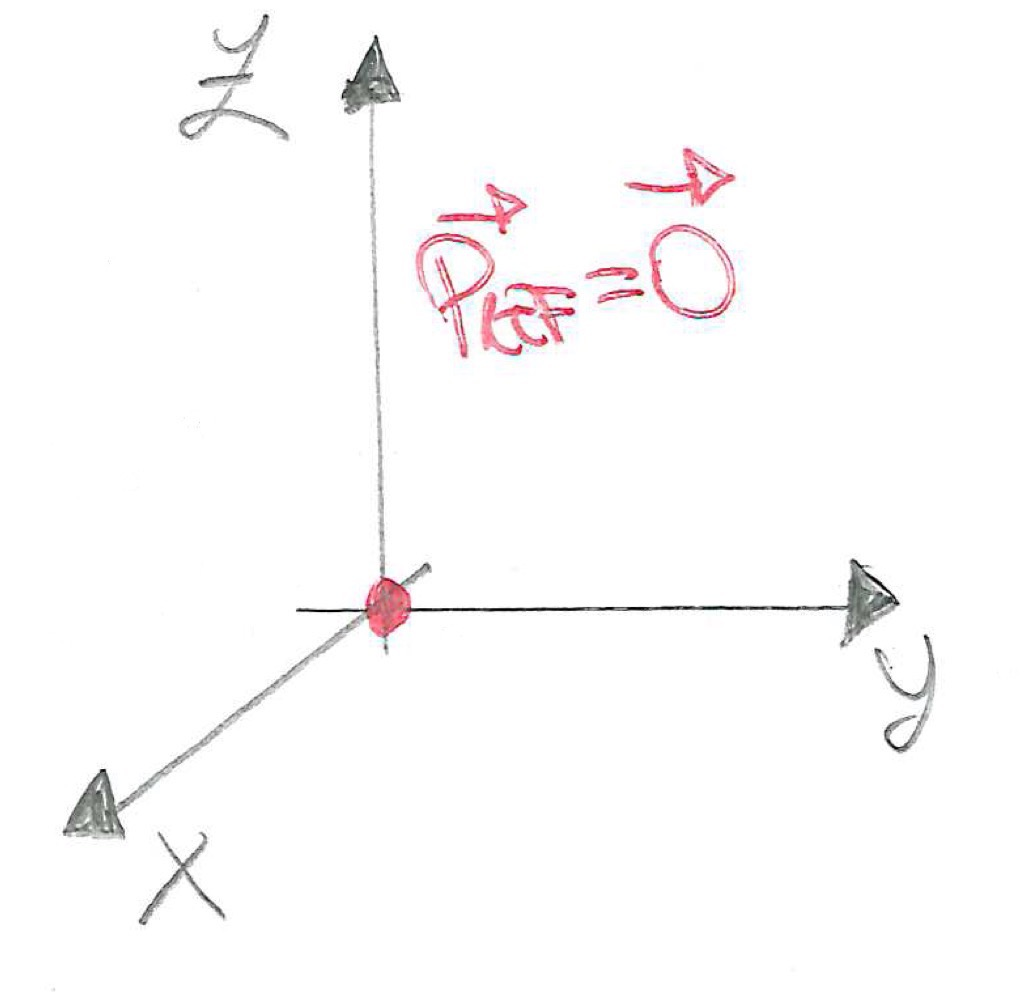
\includegraphics[]{images_ch6/rest_pcle.jpg}}
Consideriamo una particella con 3-impulso che inizialmente valga \(\Vec p_\text{ref} = 0\) ed applichiamo un boost lungo l'asse $\hat{z}$, che sappiamo (dall'esercizio \ref{ex:explicit_rotation_boost_transform}) essere esprimibile tramite una matrice:
\[
B_z(\xi) =
\begin{pmatrix}
    \cosh\xi   &   0   &   0   &   \sinh\xi\\
    0   &   1   &   0   &   0\\
    0   &   0   &   1   &   0\\
    \sinh\xi   &   0   &   0   &   \cosh\xi
\end{pmatrix}
\]
Di conseguenza, considerando \(p^\mu_\text{ref} = (M, \Vec p_\text{ref})\), abbiamo:
\[ B_z(\xi)p^\mu_\text{ref} =
\marginnote{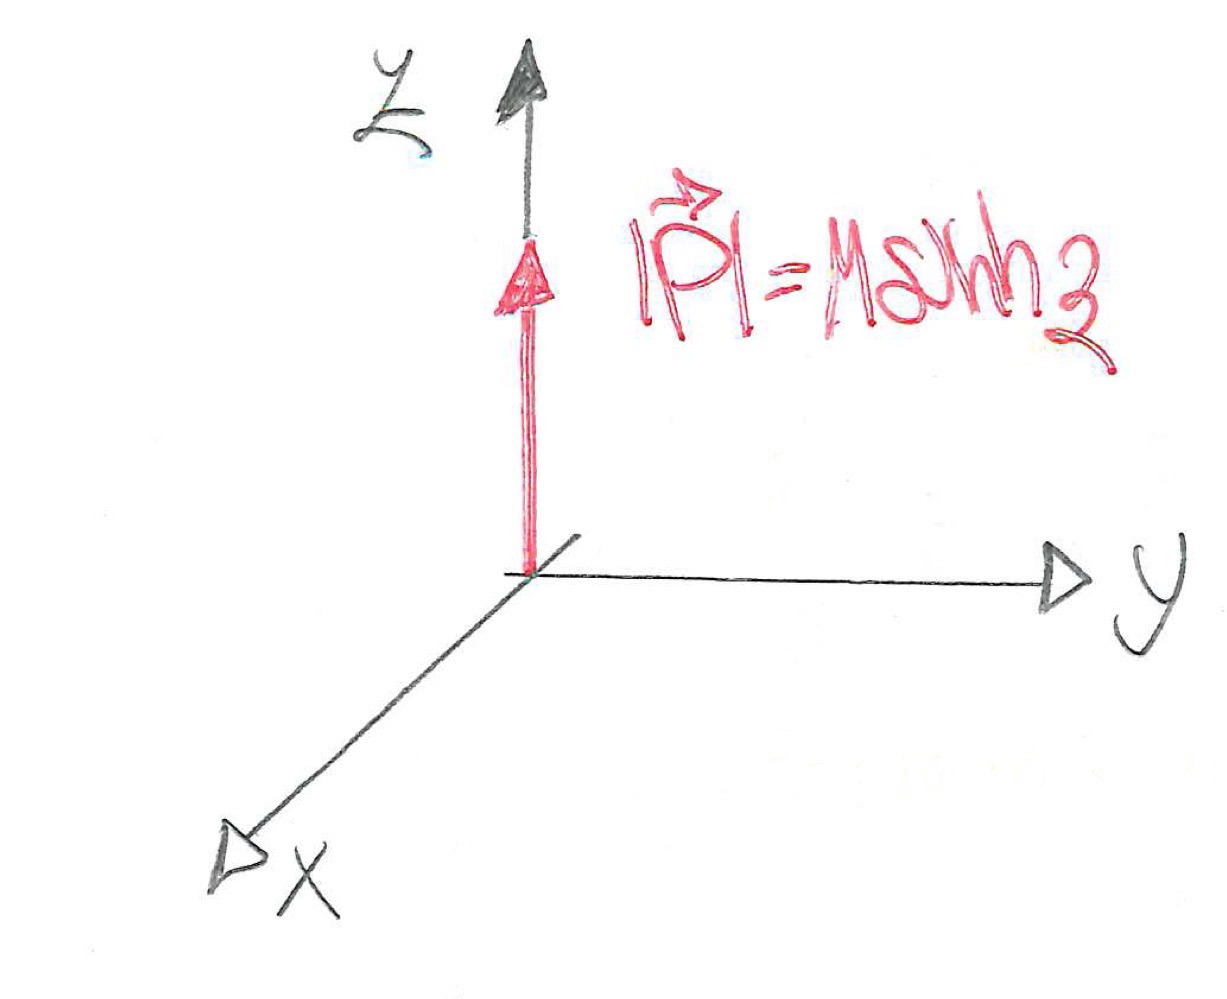
\includegraphics[]{images_ch6/boosted_pcle.jpg}}
\begin{pmatrix}
    M\cosh\xi\\     0    \\     0    \\ M\sinh\xi
\end{pmatrix}\]
Ovvero, dopo il boost la particella sviluppa un impulso $\Vec p = M\sinh\xi ~\hat{z}$.

Adesso introduciamo la matrice di rotazione \(R_{\hat{n}}\), che trasforma il versore $\hat{z}$ nel generico versore \(\hat{n} = (n_1,n_2,n_3)\) con \(n_1^2 + n_2^2 + n_3^2 = 1\):

\[
R_{\hat{n}} =
\begin{pmatrix}\begin{array}{ccc}
    1-\frac{n_1^2}{1+n_3}   &   \frac{-n_1n_2}{1+n_3}   &   n_1   \\
    \frac{-n_1n_2}{1+n_3}   &   1-\frac{n_1^2}{1+n_3}   &   n_2   \\
    -n_1                    &   -n_2                    &   n_3  
\end{array}\end{pmatrix}
\]
a cui anche in questo caso associamo la trasformazione di Lorentz:
\[
\Lambda_{R_{\hat{n}}} \equiv
\begin{pmatrix} 
\begin{array}{c|c}
    1 & \begin{array}{ccc} \phantom 0 & \phantom 0 & \phantom 0 \end{array} \\
    \hline
    \begin{array}{c} \phantom 0 \\ \phantom 0 \\ \phantom 0 \end{array} & \begin{array}{c} \vcenter{\hbox{\hspace*{7pt}\huge$R_{\hat{n}}$\hspace*{7pt}}} \end{array}
\end{array}
\end{pmatrix}
\]

A questo punto ci interessa considerare il caso in cui \(\hat{n} \equiv \hat{p} := \frac{\Vec{p}}{|\Vec{p}|} = (\hat p_x, \hat p_y, \hat p_z)\), in modo da ottenere una rotazione che porti il versore $\hat z$ nel generico versore $\hat{p}$.

Per calcolo diretto troviamo:
\marginnote{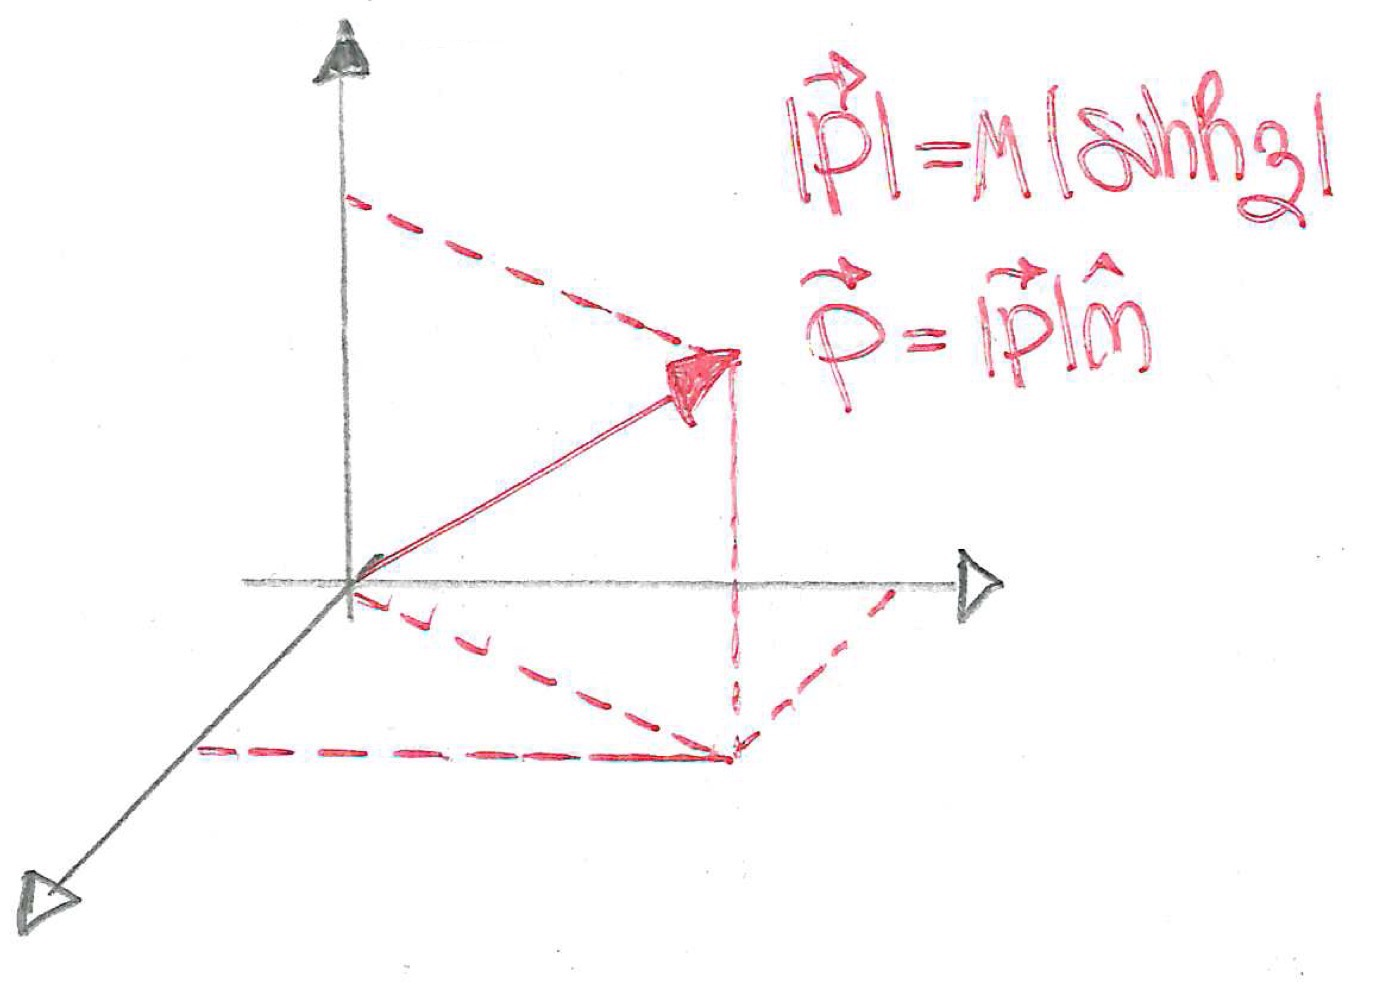
\includegraphics[]{images_ch6/rotated_boosted_pcle.jpg}}
\[
\Lambda_{R_{\hat{p}}}B_z(\xi)p_\text{ref}^\mu = \Lambda_{R_{\hat{p}}}\begin{pmatrix}M\cosh\xi\\     0    \\     0    \\ M\sinh\xi \end{pmatrix} = \begin{pmatrix}M\cosh\xi  \\ |\Vec{p}|\hat{p}  \end{pmatrix}
\]

Definiamo allora:
\[
\boxed{H\bigg(\hat{p}, \frac{|\Vec{p}|}{M}\bigg) := \Lambda_{R_{\hat{p}}}B_z\bigg(\frac{|\Vec{p}|}{M}\bigg)} \Rightarrow \boxed{p^\mu = H^\mu_{~\nu} p^\nu_\text{ref}}
\]

Introduciamo anche l'operatore \[\boxed{U_H\bigg(\hat{p}, \frac{|\Vec{p}|}{M}\bigg) \equiv U_H}\] che rappresenta l'azione di $H$ sugli stati $|M, \Vec{0}, s, \sigma\rangle$, definita da 
\[
U_H\bigg(\hat{p}, \frac{|\Vec{p}|}{M}\bigg)|M, \Vec{0}, s, \sigma\rangle \equiv U_H| \Vec{0}, \sigma\rangle
\]

Vogliamo capire come si comportano questi stati e quali sono le loro proprietà. Per farlo applichiamo $P^\mu$ a sinistra e sfruttiamo il fatto che questo trasforma come un 4-vettore sotto trasformazione di Lorentz [eq. (\ref{eq:Pmu_transform_rules})]:

\begin{align*}
    P^\mu U_H|\Vec{0}, \sigma\rangle &= U_H \overbrace{U_H^{-1} P^\mu U_H}^{H^\mu_{~\nu}P^\nu} |\Vec{0}, \sigma\rangle \\
    & = U_H H^\mu_{~\nu}P^\nu |\Vec{0}, \sigma\rangle = U_H H^\mu_{~\nu} p^\nu_\text{ref} |\Vec{0}, \sigma\rangle \\
    & = p^\mu U_H |\Vec{0}, \sigma\rangle
\end{align*}

Ci accorgiamo quindi che \(U_H\big(\hat{p}, \frac{|\Vec{p}|}{M}\big)|M, \Vec{0}, s, \sigma\rangle\) è autostato di $P^\mu$ con autovalore $p^\mu = H^\mu_{~\nu} p^\nu_\text{ref}$. In particolare, $U_H$ agisce sullo stato $|M, \Vec{0}, s, \sigma\rangle$ in modo tale da trasformare \(p_\text{ref} \rightarrow Hp_\text{ref}\), senza toccare $\sigma$.

Possiamo quindi definire il nostro stato con impulso generico:

\begin{equation}
    \boxed{|M, \Vec{p}, s, \sigma\rangle := U_H\bigg(\hat{p}, \frac{|\Vec{p}|}{M}\bigg)|M, \Vec{0}, s, \sigma\rangle}
    \label{eq:generic_momentum_state}
\end{equation}

A questo punto riscriviamo le equazioni agli autovalori, questa volta per gli stati appena costruiti. Le prime tre sono semplici, la prima la abbiamo appena dimostrata, le altre due seguono immediatamente dal fatto che \(P^2\) e \(W^2\) sono Casimir:
\[
\begin{aligned}
    &P^\mu|M, \Vec{p}, s, \sigma\rangle = p^\mu|M, \Vec{p}, s, \sigma\rangle\\
    &P^2|M, \Vec{p}, s, \sigma\rangle = M^2|M, \Vec{p}, s, \sigma\rangle\\
    &W^2|M, \Vec{p}, s, \sigma\rangle = -M^2 s(s+1)|M, \Vec{p}, s, \sigma\rangle
\end{aligned}
\]

Per quanto riguarda l'ultima c'è bisogno di una discussione apposita, che parte dalla definizione di: \marginnote{Qui stiamo utilizzando una proprietà delle trasformazioni di Lorentz, riportata ad esempio in equazione (5.9) delle \href{https://www.damtp.cam.ac.uk/user/tong/em/electro.pdf}{Lectures di David Tong} ovvero: \[(\Lambda^{-1})^\nu_{~\mu}\Lambda^\mu_{~\nu} = \delta^\nu_\nu\]}
\[
\begin{aligned}
    S^\mu_p \equiv H^\mu_{~\nu}S^\nu_\text{rest} \overset{(H^{-1})^\nu_{~\mu}\cdot}{\Longrightarrow} \big(H^{-1}\big)^\nu_{~\mu} S^\mu_p = S^\nu_\text{rest}
\end{aligned}
\]
che rende l'operatore \(\frac{S^\mu_\text{rest}W_\mu}{M} \rightarrow \frac{S^\mu_pW_\mu}{M}\).

Di conseguenza possiamo elaborare l'equazione che ci interessa come segue:
\begin{align*}
    -\frac{S^\mu_pW_\mu}{M} U_H|\Vec{0}, \sigma\rangle &= -\frac{S^\mu_p}{M} U_H \overbrace{U_H^{-1} W_\mu U_H}^{H_\mu^{~\nu}W_\nu}|\Vec{0}, \sigma\rangle \\
    &=  - U_H \frac{(H^{-1})_{~\mu}^{\nu}S^\mu_p W_\nu}{M}|\Vec{0}, \sigma\rangle = U_H \bigg(\frac{-S^\nu_\text{rest} W_\nu}{M}\bigg)|\Vec{0}, \sigma\rangle \\
    &= \sigma U_H|\Vec{0}, \sigma\rangle
\end{align*}

Si può verificare con un calcolo esplicito che l'azione di \({-S^\nu_\text{rest} W_\nu}/{M}\) su \(|M, \Vec{p}, s, \sigma\rangle\) è equivalente a quella dell'operatore \({\Vec{J}\cdot \Vec{P}}/{|\Vec{p}|}\). Questa equivalenza ci permette di riscrivere le equazioni agli autovalori nel modo seguente:

\begin{equation}
    \boxed{
        \begin{aligned}
            &P^\mu|M, \Vec{p}, s, \lambda\rangle = p^\mu~|M, \Vec{p}, s, \lambda\rangle\\
            &P^2|M, \Vec{p}, s, \lambda\rangle = M^2~|M, \Vec{p}, s, \lambda\rangle\\
            &W^2|M, \Vec{p}, s, \lambda\rangle = -M^2 s(s+1)~|M, \Vec{p}, s, \lambda\rangle\\
            &{\Vec{J}\cdot \Vec{P}}|M, \Vec{p}, s, \lambda\rangle = \lambda|\Vec{p}|~|M, \Vec{p}, s, \lambda\rangle
        \end{aligned}
        }~,~ \text{con} \quad
        \begin{aligned}
            &s=0,\frac{1}{2},1,\frac{3}{2},\cdots\\
            &-s<\lambda<s
        \end{aligned}
    \label{eq:final_eigensystem_massive}
\end{equation}
Notiamo la sostituzione \(\sigma\leftrightarrow\lambda\) interpretata come elicità, in quanto stiamo estraendo la componente dello spin totale $\Vec{J}$ parallela alla direzione del moto, i.e. l'elicità. In particolare se scriviamo $\Vec{J} = \Vec{L}+ \Vec{S}$, allora lungo la direzione del moto, che è planare in quanto diretto come $\hat z$, sopravvive solo lo spin e l'elicità $\lambda = \Vec{J}\cdot\Vec{p}/|\Vec{p}|$ rappresenta la proiezione dello spin lungo la direzione del moto.

\begin{exercise}
    Calcolare esplicitamente \(-S_p^\mu W_\mu/M |M, \Vec{0}, s, \sigma\rangle\). \textbf{[Conti svolti Lez. 23 p. 47÷49]}
\end{exercise}

\subsection{Step 6}

Vogliamo dimostrare la seguente affermazione:
\begin{kaobox}
    Il sottospazio \(\big\{ |M,\Vec{p},s,\lambda\rangle \big\}\), con massa $M$ e spin $s$ fissati, fornisce una rappresentazione unitaria e irriducibile (\textbf{R.U.I.}) del gruppo di Poincaré.
\end{kaobox}
\begin{proof} Per dimostare la nostra tesi, sfruttiamo l'azione di un generico elemento del gruppo\footnote{Qui c'è ovviamente un abuso di notazione, parliamo di elemento del gruppo ma ci stiamo riferendo alla rappresentazione dello stesso.} di Poincaré: \(U(\Lambda, a) = U(\mathbb 1, a)U(\Lambda, 0) \).

\begin{itemize}
    \item Consideriamo prima le traslazioni. Per mezzo della mappa esponenziale dei generatori abbiamo 
    \[U(\mathbb 1, a) = e^{ia_\mu P^\mu} \Rightarrow 
    \boxed{U(\mathbb 1, a)|M,\Vec{p},s,\lambda\rangle = e^{ia_\mu p^\mu}|M,\Vec{p},s,\lambda\rangle}\]

    \item Consideriamo ora le trasformazioni di Lorentz e per amor di notazione chiamiamo $U_\Lambda\equiv U(\Lambda, 0)$. 

    Il nostro obiettivo è calcolare \(U_\Lambda|M,\Vec{p},s,\lambda\rangle\), ma prima di tutto ci accorgiamo di quanto segue:
    \begin{align*}
        P_\mu U_\Lambda|M,\Vec{p},s,\lambda\rangle &=U_\Lambda U_\Lambda ^{-1} P^\mu U_\Lambda |M,\Vec{p},s,\lambda\rangle\\
        &= U_\Lambda \Lambda^\mu_{~\nu}P^\nu |M,\Vec{p},s,\lambda\rangle\\
        &=U_\Lambda \Lambda^\mu_{~\nu}p^\nu |M,\Vec{p},s,\lambda\rangle\\
        &=p_\Lambda^\mu U_\Lambda |M,\Vec{p},s,\lambda\rangle
    \end{align*}
    In altre parole \(U_\Lambda|M,\Vec{p},s,\lambda\rangle\) è ancora autostato di $P^\mu$ con autovalore $p_\Lambda^\mu \equiv \Lambda^\mu_{~\nu}p^\nu$.

    Ha quindi senso definire: \[|M,\Vec{p}_\Lambda,s,\lambda\rangle = U_H\Big(\hat{p}_\Lambda, \frac{|\Vec{p}_\Lambda|}{M}\Big)|M,\Vec{0},s,\lambda\rangle\]

    dove ad $U_H$ è associata una trasformazione $H\big(\hat{p}_\Lambda, \frac{|\Vec{p}_\Lambda|}{M}\big)$ che trasforma il vettore di riferimento nel 4-vettore $p_\Lambda^\mu$ con componente spaziale $\Vec{p}_\Lambda$.

    Torniamo ora al nostro obiettivo iniziale ed operiamo nel modo seguente:
    \begin{align*}
        U_\Lambda|M,\Vec{p},s,\lambda\rangle &= U_\Lambda U_H\Big(\hat{p}, \frac{|\Vec{p}|}{M}\Big)|M,\Vec{0},s,\lambda\rangle \\
        &= U_H\Big(\hat{p}_\Lambda, \frac{|\Vec{p}_\Lambda|}{M}\Big)U_H\Big(\hat{p}_\Lambda, \frac{|\Vec{p}_\Lambda|}{M}\Big)^{-1}U_\Lambda U_H\Big(\hat{p}, \frac{|\Vec{p}|}{M}\Big)|M,\Vec{0},s,\lambda\rangle\\
    \end{align*}

    Nello spazio dell'impulso, abbiamo:
    \[
    p_\text{ref}^\mu \xrightarrow[]{H(\hat{p}, \nicefrac{|\Vec{p}|}{M})} p^\mu = H^\mu_{~\nu}p^\nu_\text{ref}
    \xrightarrow[]{\Lambda} p_\Lambda^\mu = \Lambda^\mu_{~\nu}p^\nu
    \xrightarrow[]{H(\hat{p}_\Lambda, \nicefrac{|\Vec{p}_\Lambda|}{M})^{-1}} p_\text{ref}^\mu
    \]

    quindi \(p_\text{ref}^\mu\) è invariante sotto azione dell'operatore \(H(\hat{p}_\Lambda, \nicefrac{|\Vec{p}_\Lambda|}{M})^{-1}\Lambda H(\hat{p}, \nicefrac{|\Vec{p}|}{M})\), il che rende tale operatore un elemento del piccolo gruppo, i.e. una rotazione. Nello specifico è una \textbf{rotazione di Wigner}:
    \begin{equation}
        \boxed{
        \omega(\Lambda, p) = H(\hat{p}_\Lambda, \nicefrac{|\Vec{p}_\Lambda|}{M})^{-1}\Lambda H(\hat{p}, \nicefrac{|\Vec{p}|}{M})
        }
        \label{eq:wigner_rotation}
    \end{equation}

    Di conseguenza, abbiamo l'operatore che descrive l'azione della rotazione di Wigner sugli stati $|M,\Vec{0},s,\lambda\rangle$:

    \begin{equation}
        \boxed{
        U_\omega(\Lambda, p) = U_H(\hat{p}_\Lambda, \nicefrac{|\Vec{p}_\Lambda|}{M})^{-1} U_\Lambda U_H(\hat{p}, \nicefrac{|\Vec{p}|}{M})
        }
        \label{eq:wigner_rotation_operator}
    \end{equation}

    Ma per quanto visto in precedenza, sappiamo come agiscono le rotazioni su questi stati: lo fanno secondo l'equazione (\ref{eq:rotation_operator_action}). Possiamo quindi applicarla al nostro caso:
    \begin{align*}
        U_\Lambda|M,\Vec{p},s,\lambda\rangle &=  U_H\Big(\hat{p}_\Lambda, \frac{|\Vec{p}_\Lambda|}{M}\Big)  \overbrace{\Big[D_s\big(\omega(\Lambda, p)\big)\Big]_{\lambda'\lambda} |M,\Vec{0},s,\lambda'\rangle}^{U_\omega(\Lambda, p)|M,\Vec{0},s,\lambda\rangle} \\
        &= \Big[D_s\big(\omega(\Lambda, p)\big)\Big]_{\lambda'\lambda} |M,\Vec{p}_\Lambda,s,\lambda'\rangle
    \end{align*}
\end{itemize}
In conclusione, sotto una generica trasformazione di Poincaré:
\begin{equation}
    \boxed{\begin{aligned}
    U(\Lambda,a)|M,\Vec{p},s,\lambda\rangle &= U(\mathbb 1, a)U(\Lambda, 0) |M,\Vec{p},s,\lambda\rangle =\\
    &=e^{ia_\mu p_\Lambda^\mu}\Big[D_s\big(\omega(\Lambda, p)\big)\Big]_{\lambda'\lambda} |M,\Vec{p}_\Lambda,s,\lambda'\rangle
    \end{aligned}}
    \label{eq:poincare_action_generic_state_massive}
\end{equation}

E fondamentalmente abbiamo finito, infatti:
\begin{itemize}
    \item[\blacksquare] L'equazione (\ref{eq:poincare_action_generic_state_massive}) definisce completamente l'azione di una qualunque trasformazione di Poincaré generica sugli stati $|M,\Vec{p},s,\lambda\rangle$ nel sottospazio da essi generato quando $M$ ed $s$ sono fissati.

    \item[\blacksquare] La mappa \(P(\Lambda,a) \rightarrow U(\Lambda,a)\) così definita è un omomorfismo su \(\Big\{|M,\Vec{p},s,\lambda\rangle\Big\}\).

    \item[\blacksquare] \textbf{La rappresentazione fornita da $\mathbf{U(\Lambda,a)}$ è unitaria} ed è immediato verificarlo, in quanto nella (\ref{eq:poincare_action_generic_state_massive}) abbiamo un esponenziale complesso, che è unitario, e le matrici \(\Big[D_s\big(\omega(\Lambda, p)\big)\Big]_{\lambda'\lambda}\), anch'esse unitarie in quanto rappresentano rotazioni ordinarie.

    \item[\blacksquare] \textbf{Le rappresentazioni fornite da $\mathbf{U(\Lambda,a)}$} nei sottospazi \(\Big\{|M,\Vec{p},s,\lambda\rangle\Big\}_{M,s}\) \textbf{sono anche irriducibili}, secondo la seguente definizione:
    \begin{definition}
        \textbf{(Rappresentazione Irriducibile.)}
        
        Una rappresentazione \(D~:~ G\rightarrow \text{GL}(V)\) si dice irriducibile se \textbf{non} c'è alcun sottospazio non-banale di $V$ che sia invariante sotto l'azione di $G$ per mezzo di $D$ per ogni $g\in G$ (i.e. è irriducibile se al più ammette i sottospazi invarianti banali, $\{\varnothing\}$ e $V$ stesso).
        \label{def:irrep}
    \end{definition}
    Nel nostro caso infatti, non è possibile definire alcun sottospazio invariante, in quanto tutti i vettori in \(\Big\{|M,\Vec{p},s,\lambda\rangle\Big\}_{M,s}\) sono connessi da una trasformazione di Poincaré.
\end{itemize}
\end{proof}

Abbiamo quindi le seguenti rappresentazioni irriducibili (abbreviato \textbf{irreps}), suddivise nello stesso modo che abbiamo visto alla fine dello step 4, ad ogni colonna corrisponde una irrep:
\begin{center}
    \begin{tabular}{|l|l|l|l|}
    \textit{Scalare Massivo}               & \textit{Fermione Massivo}                    & \textit{Vettore Massivo} \\
    \hline
    $M, s=0$                      &   $M, s=\nicefrac{1}{2}$            &   $M, s=1$                      & $\cdots$  \\
    \hline
    \(|M, \Vec{0}, 0, 0\rangle\)    &   \(|M, \Vec{0}, \frac{1}{2}, +\frac{1}{2}\rangle\)    &   \(|M, \Vec{0}, 1, 1\rangle\)    & \\
                                    &   \(|M, \Vec{0}, \frac{1}{2}, -\frac{1}{2}\rangle\)    &   \(|M, \Vec{0}, 1, 0\rangle\)    & \\
                                    &                                                        &   \(|M, \Vec{0}, 1, -1\rangle\)   & \\ \hline
    \end{tabular}
\end{center}
\textbf{Ogni rappresentazione irriducibile è uno stato di singola particella}, e.g. la prima colonna corrisponde allo stato di singola particella di impulso $\Vec{p}$, massa $M$ e spin $0$, i.e. uno stato \textit{scalare massivo}. Questo significa che siamo molto vicini a ciò che, in apertura del capitolo, abbiamo definito come il nostro scopo principale: caratterizzare gli stati multi-particellari $|\psi\rangle$ ed implementare le trasformazioni di Poincaré rappresentandole con operatori unitari, in modo tale da rendere le probabilità di transizione invarianti sotto il cambio di sistema di riferimento.

È interessante notare che:
\begin{itemize}
    \item \textbf{Una particella massiva di spin “$\mathbf{s}$” ha $\mathbf{2s+1}$ gradi di libertà}, ovvero gli stati di elicità nella base che abbiamo costruito. Questo è vero in $\mathsf d = 4$ dimensioni e per i fermioni massivi notiamo che ogni stato ha 2 gradi di libertà. Di norma si pensa ai fermioni come stati con 4 gradi di libertà, e questi sono rispettati quando si considerano entrambi gli stati nella rappresentazione.
    \item Per una particella massiva, \textbf{l'elicità è un invariante di Lorentz}.
\end{itemize}

\section{Un commento tecnico}
\textbf{Nota: } \textit{Questa sezione non ha lo scopo di essere esaustiva, per i dettagli ci si può riferire alla Lezione 24 pag. 57÷62.}

\textbf{Lo step 5 non è unico}. È infatti possibile generare un impulso \(\Vec{p}\) partendo da \(\Vec{p}_\text{ref}\) in svariati modi ed ognuno produce di conseguenza una base differente. Noi abbiamo scelto quello che alla fine dei conti ci ha permesso di identificare \(\sigma\) nello stato in moto con l'elicità, la cosiddetta “base di elicità” ma è possibile ricavare, in modo simile rispetto a quello che abbiamo sviluppato nel dettaglio, un'altra base con un significato fisico rilevante: la “base di polarizzazione di spin”, in cui $\sigma$ nello stato in moto è identificata come la terza componente dello spin (o in altri termini la proiezione dello spin lungo la direzione $\hat z$).

Questa è la base che adotta ad esempio il libro di Weinberg ed in sostanza basa la sua derivazione sulla scelta di un particolare boost nella direzione specificata da $\nicefrac{\Vec{p}}{|\Vec{p}|}$, $L(\Vec{p},M)$, diverso dalla trasformazine $H(\hat{p}, \nicefrac{|\Vec{p}|}{M})$ che abbiamo scelto noi e definito come segue:
\begin{equation}
    L(\Vec{p},M) = 
    \begin{pmatrix}
    \begin{array}{cc}
        \nicefrac{p^0}{M}   &   -\nicefrac{p_j}{M} \\
        \nicefrac{p^i}{M}   &   \delta^i_j -\frac{p^ip_j}{M(p^0+M)}
    \end{array}
    \end{pmatrix}
    \label{eq:boost_def_spinpol_basis}
\end{equation}
Da qui in poi bisogna semplicemente svolgere gli stessi passaggi che abbiamo effettuato nello step 5 definendo l'operatore associato al boost, che in questo caso comprende già una rotazione implicita al suo interno, e ridefinendo l'operatore \(-S^\mu_\text{rest}W_\mu/M\) per mezzo di \(S_L^\mu=L^\mu_{~\nu}S^\nu_\text{rest}\).

Il punto chiave che permette l'identificazione di \(\sigma\) nello stato in moto con la terza componente dello spin è lo stesso in cui abbiamo scoperto che \(S_L^\mu W_\mu\) corrispondeva (a meno di fattori qui non riportati) all'operatore di elicità. Sviluppando il prodotto si trova che in questo caso:
\[
-\frac{S^\mu_\text{rest}W_\mu}{M} = +\frac{1}{M}(L^{-1})^3_{~\mu}W^\mu
\]
e posto \(J_s^k = \frac{1}{M}\big[L(\Vec{p}, M)^{-1}\big]^k_{\mu}W^\mu\) si arriva all'ultima equazione dell'auto-sistema scritta nel modo seguente:
\[
J^3_s|M, \Vec{p}, s, \sigma\rangle = \sigma|M, \Vec{p}, s, \sigma\rangle 
\]

Il punto un po' contorto e che quindi rende più “fisicamente chiaro” il nostro approccio è il fatto che, per accorgerci dell'identificazione $\sigma\leftrightarrow $ spin lungo $\hat{z}$, bisogna tirare in causa l'algebra di $\text{SU}(2)$, che è la stessa sia per il momento angolare orbitale che per lo spin, in quanto $\Vec{J}_s$ chiude tale algebra. 

Tuttavia si verifica che $\big[J_s^i, P^k\big]=0$, il che identifica $\Vec{J}_s$ con il vettore di spin, dato che il momento angolare orbitale non commuta con la quantità di moto.

Il completo auto-sistema, nella base di polarizzazione di spin, si scrive:

\begin{equation}
    \boxed{
        \begin{aligned}
            &P^\mu|M, \Vec{p}, s, \sigma\rangle = p^\mu_\text{ref}~|M, \Vec{p}, s, \sigma\rangle\\
            &P^2|M, \Vec{p}, s, \sigma\rangle = M^2~|M, \Vec{p}, s, \sigma\rangle\\
            &W^2|M, \Vec{p}, s, \sigma\rangle = -M^2 s(s+1)~|M, \Vec{p}, s, \sigma\rangle\\
            &J^3_s|M, \Vec{p}, s, \sigma\rangle = \sigma~|M, \Vec{p}, s, \sigma\rangle
        \end{aligned}
        }~,~ \text{con} \quad
        \begin{aligned}
            &s=0,\frac{1}{2},1,\frac{3}{2},\cdots\\
            &-s<\sigma<s
        \end{aligned}
    \label{eq:final_eigensystem_massive_weinberg}
\end{equation}


Dal resto del procedimento emerge invece una semplificazione, collegata alla rotazione di Wigner, in questo caso definita da:

\[
\omega_L(\Lambda, p) = L(\Vec{p}_\Lambda,M)^{-1} \Lambda L(\Vec{p},M) ~~\in \text{SO}(3)
\]
Tale rotazione comporta la seguente azione del generico elemento del gruppo di Poincaré per mezzo della rappresentazione $U$ sugli stati $|M, \Vec{p}, s, \sigma\rangle$:
\[
U(\Lambda,a)|M,\Vec{p},s,\sigma\rangle =e^{ia\cdot p_\Lambda}\Big[D_s\big(\omega_L(\Lambda, p)\big)\Big]_{\sigma'\sigma} |M,\Vec{p}_\Lambda,s,\sigma'\rangle
\]

Tuttavia, c'è un teorema (che non dimostreremo) valido in questo caso\footnote{Dalla dimostrazione si capisce perché questo teorema sia valido solo per rotazioni di Wigner costruite per mezzo di soli boost}, che dice quanto segue e che semplifica notevolmente la rotazione di Wigner:
\begin{theorem}
    Sia $\Lambda=\Lambda_R \in \pazocal L = \text{SO}^+(1,3)$ una rotazione pura, allora una rotazione di Wigner ad essa associata costruita per mezzo di soli boost è \(\Lambda_R\) stessa, i.e.:
    \[
    \omega_L(\Lambda_R, p) = \Lambda_R
    \]
    \label{th:wigner_rot_pure_rot}
\end{theorem}

\section{R.U.I. di $\mathbf{\pazocal P}$ nel caso massless}

Nel processo di costruzione delle rappresentazioni unitarie irriducibili del gruppo di Poincaré, in particolare alla fine dello step 2, abbiamo scelto di trattare il caso di particella massiva. Discutiamo invece adesso il caso di particella non massiva (o massless), i.e. consideriamo il caso in cui $p^2=0$ con $p^0 = |\Vec{p}| > 0$.

Sulla base di tale assunzione, rivisitiamo alcuni dei passaggi che abbiamo già svolto.

\subsection{Step 3}

Chiaramente avremo bisogno di un \textbf{vettore di riferimento differente}, in quanto per una particella non massiva, come ad esempio un fotone, non esiste alcuno stato a riposo. Ovviamente la scelta è del tutto arbitraria, ma la nostra scelta sarà la seguente:

\[
\boxed{p^\mu_\text{ref} = (k,0,0,k)~,\quad k>0}
\]

Di conseguenza, le equazioni agli autovalori in questo caso saranno:
\[
\boxed{
    \begin{aligned}
        &P^\mu|0, k\hat{z}\rangle = p^\mu_\text{ref}|0, k\hat{z}\rangle\\
        &P^2|0, k\hat{z}\rangle = 0
    \end{aligned}
}
\]
dove manteniamo l'autovalore\footnote{A meno del quadrato, ovviamente} di $P^2$, $M=0$, come “etichetta” nello stato per evidenziare che siamo nel caso massless.

\subsection{Step 4}
Rivisitiamo a questo punto il \textbf{gruppo piccolo} per $p^\mu_\text{ref}$. Se nel caso massivo la scelta del gruppo delle rotazioni, $\text{SO}(3)$, era quasi telegrafata, in questo caso la situazione è un po' differente.
\marginnote{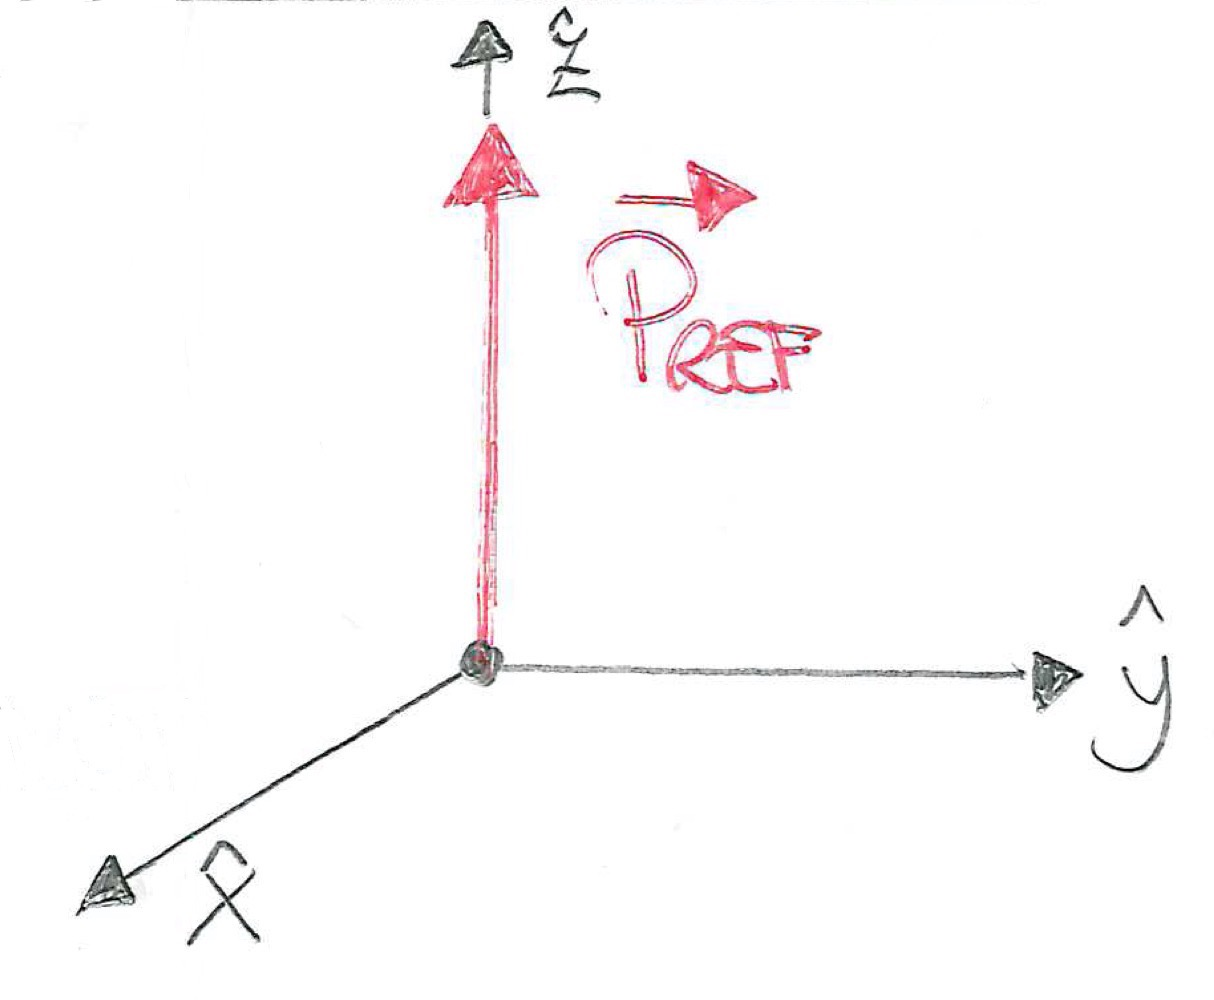
\includegraphics[]{images_ch6/massless_refvector.jpg}}

Questa volta abbiamo a che fare con un vettore di riferimento che presenta un impulso iniziale diretto come $\hat{z}$ ed intuitivamente, ruotando nel piano $(x,y)$ attorno $\hat{z}$, allora $p^\mu_\text{ref}$ resta invariato. Tuttavia, nel gruppo piccolo di questo $p^\mu_\text{ref}$ esistono trasformazioni più generali delle semplici rotazioni attorno l'asse $z$, identificabili con $\text{SO}(2)$.

Per determinare quale sia il gruppo piccolo che stiamo cercando, ci avvaliamo del seguente teorema:
\begin{theorem}
    \textbf{(Generatori del gruppo piccolo.)}

    Sia $\mathscr G(p^\mu_\mathrm{ref})$ il gruppo delle trasformazioni di Lorentz sotto cui $p^\mu_\mathrm{ref}$ è invariante, i.e. il suo gruppo piccolo. 

    Allora $\mathscr G(p^\mu_\mathrm{ref})$ è generato dalle tre componenti del seguente vettore:
    \begin{equation}
        \boxed{\Vec{T} = \Vec{J}_\mathrm{vec} + \frac{\Vec{K}_\mathrm{vec}\times\Vec{p}_\mathrm{ref}}{p^0_\mathrm{ref}}}
        \label{eq:littlegroup_gens}
    \end{equation}
    dove $\Vec{J}_\mathrm{vec}$ e $\Vec{K}_\mathrm{vec}$ sono, rispettivamente, i generatori di rotazioni e boost nella notazione vettoriale ricavata nell'esercizio \ref{ex:vec_generators_form}.
    \label{th:littlegroup_gens}
\end{theorem}

\begin{exercise}
    Dimostrare il Teorema \ref{th:littlegroup_gens}. \textbf{[Conti svolti Lezione 24 pag. 64÷67]}
\end{exercise}

\begin{nota}
    Il Teorema \ref{th:littlegroup_gens} vale in generale! Nel caso massivo, in cui $p^\mu_\text{ref} = \big(M,0\big)$, i generatori $\Vec{T}\equiv\Vec{J}_\mathrm{vec}$, il che significa che il gruppo piccolo è $\text{SO}(3)$, come trovato in precedenza.  
\end{nota}

Essendo \(\nicefrac{\Vec{p}_\mathrm{ref}}{p^0_\mathrm{ref}} = \hat{z}\), possiamo scrivere le componenti dei generatori del gruppo piccolo come segue:
\begin{equation}
    \begin{aligned}
        &T_x \equiv  J^1_\mathrm{vec} + K^2_\mathrm{vec}\\
        &T_y \equiv  J^2_\mathrm{vec} - K^1_\mathrm{vec}\\
        &T_z \equiv  J^3_\mathrm{vec} 
    \end{aligned}
    \label{eq:littlegroup_gens_components}
\end{equation}
In $J^3_\mathrm{vec}$ riconosciamo il generatore delle rotazioni attorno all'asse $\hat{z}$, ovvero del gruppo $\text{SO}(2)$, e questo ci dice quello che abbiamo già anticipato: $\mathscr G (p_\text{ref})$ è necessariamente più grande di $\text{SO}(2)$.

In particolare, si può dimostrare che tra i generatori, espressi come in equazione (\ref{eq:littlegroup_gens_components}), valgono le seguenti relazioni di commutazione:
\begin{equation}
    \big[T_x, T_y\big] = 0 \quad \big[T_z, T_x\big] = iT_y \quad \big[T_z, T_y\big] = -iT_x
    \label{eq:E2_algebra}
\end{equation}

E questa non è nient'altro se non l'algebra del gruppo euclideo in due dimensioni, i.e. $E(2)$. Ovvero il gruppo delle trasformazioni sotto cui è invariante la metrica euclidea.

\begin{exercise}
    Dimostare che i generatori del gruppo piccolo (\ref{eq:littlegroup_gens_components}) chiudono l'algebra di $E(2)$ (\ref{eq:E2_algebra}). \textbf{[Conti svolti Lezione 24 pag. 68]}
\end{exercise}

Di conseguenza \textbf{il gruppo piccolo nel caso massless è $E(2)$} ed è giunto il momento di ripetere le operazioni svolte nel caso massivo, ovvero aggiungere etichette agli stati $|0,k\hat{z}\rangle$ per descrivere come questi trasformano sotto gli elementi del gruppo piccolo.

Siccome nel caso massivo abbiamo usato il Casimir di ${SO}(3)$\footnote{\textbf{Attenzione:} gli operatori di Casimir sono elementi dell'algebra di $\text{SO}(3)$, in notazione matematica indicata con $\mathfrak{so}(3)$, che in notazione fisica si confonde con il gruppo.}, $|\Vec{J}|^2$, e l'operatore $J^3$. Con lo stesso spirito \textbf{proviamo innanzitutto ad utilizzare il Casimir di $\mathbf{E(2)}$}, fornito dall'operatore \(T_x^2 + T_y^2\) (analogo di $P^2$ ma per le rotazioni bi-dimensionali sul piano euclideo). 
\begin{nota}
    L'unica relazione di commutazione non banale da dimostrare per verificare che \(T_x^2 + T_y^2\) sia un Casimir è quella con $T_z$:
    \[
    \begin{aligned}
        \big[T_z, T_x^2 + T_y^2\big] &= T_x\big[T_z, T_x\big] +\big[T_z, T_x\big]T_x + T_y\big[T_z, T_y\big] +\big[T_z, T_y\big]T_y = \\
        &= iT_xT_y +iT_yT_x - iT_yT_x  - iT_xT_y =\\  
        &= 0
    \end{aligned}
    \]\qed
\end{nota}

Siamo a questo punto tentati dallo scrivere le equazioni agli autovalori nel modo seguente:

\[
{
\begin{aligned}
    &P^\mu|0, k\hat{z}, w\rangle = p^\mu_\text{ref}|0, k\hat{z}, w\rangle\\
    &P^2|0, k\hat{z}, w\rangle = 0 \\
    &(T_x^2 + T_y^2)|0, k\hat{z}, w\rangle = w |0, k\hat{z}, w\rangle
\end{aligned}
}
\]

Per farlo dobbiamo prima verificare che \((T_x^2 + T_y^2)\) e \(P^\mu\) commutino tra loro, il che permette di diagonalizzarli insieme.

Se ci restringiamo al sottospazio di $p_\text{ref}$, ossia quello generato dai vettori \(|0, k\hat{z}, w\rangle\) facciamo una scoperta interessante. Riprendiamo lo pseudovettore di Pauli-Lubanski, le cui componenti nel sottospazio considerato diventano:
\[
\begin{cases}
    W^0 = \Vec{J}\cdot\Vec{P} \\
    \Vec{W} = P^0\Vec{J} + \Vec{K}\times\Vec{P}
\end{cases}
\rightarrow
\begin{cases}
    W^0 = J^3 k \\
    \Vec{W} = k\big(\Vec{J} + \Vec{K}\times\hat{z}\big) \overset{\text{\ref{eq:littlegroup_gens}}}{=} k\Vec{T}
\end{cases}
\]

\textbf{La componente spaziale del vettore di Pauli-Lubanski}, ristretta al sottospazio di $p^\mu_\text{ref}$, \textbf{è un multiplo dei generatori dell'algebra di $\mathbf{E(2)}$}.

Ne consegue che:
\[
W^2 = (W^0)^2 - |\Vec{W}|^2 = -k^2(T_x^2 + T_y^2)
\]
Ma allora, sempre nel sottospazio del vettore di riferimento, possiamo scrivere l'ultima equazione nel modo seguente:
\[
\boxed{-\frac{W_\mu W^\mu}{k^2}|0, k\hat{z}, w\rangle = w |0, k\hat{z}, w\rangle}
\]
Che ci facilita anche la generalizzazione ad impulso qualunque in quanto presenta il Casimir di $\pazocal P$, $W^2$, che abbiamo già incontrato.

Dobbiamo ora specificare come gli stati trasformino sotto gli elementi di $\text{SO}(2)$, i.e. quelli generati da $J^3$. Nel sottospazio del vettore di riferimento $P^\mu$ e $J^3$ commutano, in quanto in generale tra i due vale la relazione \(\big[J^3, P^k\big] = i\varepsilon^{3ik}P^k\), ma $P^3$ è l'unica componente diversa da zero in tale sottospazio e $\varepsilon^{3i3}=0$.

Possiamo diagonalizzare anche $J^3$ insieme agli altri tre operatori, non resta che trovare l'equazione agli autovalori anche per quest'ultimo.

\begin{nota}
    L'operatore $J^3$ genera rotazioni 1-dimensionali attorno a $\hat{z}$, le quali compongono il gruppo $\text{SO}(2) < \text{SO}(3)$. Un elemento $R(\phi) \in \text{SO}(2)$ è specificato da un singolo parametro $phi\in[0,2\pi)$, l'angolo della rotazione. 
    \begin{itemize}
        \item Il gruppo è abeliano.
        \item La regola di composizione è \(R(\phi_1) R(\phi_2) = R(\phi_1 + \phi_2)\), corredata dalla condizione $R(\phi) = R(\phi \pm 2\pi)$ se $\phi$ è fuori dall'intervallo $[0,2\pi)$.
        \item L'elemento neutro è $R(0) = \mathbb 1$.
        \item L'elemento inverso è $R(\phi)^{-1} = R(-\phi)$
    \end{itemize}
    \label{note:SO2}
\end{nota}

Essendo $\text{SO}(2)$ abeliano, per il lemma di Schur le sue rappresentazioni irriducibili complesse sono 1-dimensionali. Per cercare tali rappresentazioni partiamo dall'algebra e consideriamo l'equazione agli autovalori per $J^3$:
\[
J^3|\lambda\rangle = \lambda|\lambda\rangle
\]
dove $\lambda \in \mathbb R$ in quanto, visto che stiamo cercando rappresentazioni unitarie, $J^3$ deve essere Hermitiana.

A questo punto, sappiamo di poter ottenere gli elementi del gruppo per mezzo della mappa esponenziale \(U(\phi) = \exp(-i\phi J^3)\). Di conseguenza avremo:
\[
U(\phi)|\lambda\rangle = e^{-i\phi J^3}|\lambda\rangle = e^{-i\phi \lambda}|\lambda\rangle
\]
Imponendo ora la condizione supplementare della legge di composizione di $\text{SO}(2)$, citata nella nota \ref{note:SO2}, arriviamo al seguente risultato:
\[
 e^{-i\phi \lambda}|\lambda\rangle = e^{-i\phi \lambda}e^{\mp i2\pi\lambda}|\lambda\rangle 
\]
Ma allora, siccome primo ed ultimo membro devono essere uguali, \(e^{\mp i2\pi\lambda} \overset{!}{=}1\), da cui segue che necessariamente $\lambda\in \mathbb Z = 0, \pm1, \pm2,...$ .

Le rappresentazioni irriducibili \textit{ordinarie} di $\text{SO}(2)$ sono quindi definite da 
\[
\boxed{J^3|\lambda\rangle = \lambda|\lambda\rangle~,\quad\lambda\in\mathbb Z}
\]

Ma non abbiamo ancora finito: tutto questo discorso ha lo scopo di essere applicato in un contesto quanto-meccanico, quindi \textbf{dobbiamo considerare anche le rappresentazioni proiettive di $\textbf{SO}\mathbf{(2)}$, in cui $\mathbf{\lambda}$ è semintero}.

\begin{nota}
    Come dimostrazione che le rappresentazioni con ${\lambda}$ semintero sono proiettive, consideriamo \(\lambda = \nicefrac{(2n+1)}{2}\) e l'operatore \(U(\phi) = \exp(-i\phi\nicefrac{(2n+1)}{2})\). 
    
    Presi due angoli $\phi_{1,2}$ la cui somma sia pari a $2\pi$, troviamo che
    \[
    U(\phi_1)U(\phi_2)=U(\phi_1+\phi_2) = U(2\pi) = U(2\pi-2\pi) = \mathbb 1
    \]

    D'altro canto, nella nostra rappresentazione:
    \[
    U(2\pi) = e^{-i2\pi\frac{(2n+1)}{2}} = e^{-i(2n+1)\pi}= -\mathbb 1 = e^{i\pi}\mathbb 1
    \] 

    I risultati sono uguali a meno di una fase, quindi la rappresentazione è proiettiva. \qed
    \label{note:halfint_SO2_irreps}
\end{nota}

Arriviamo quindi al sistema di equazioni seguente:
\[
{
\begin{aligned}
    P^\mu&|0, k\hat{z}, w, \lambda\rangle = p^\mu_\text{ref}|0, k\hat{z}, w, \lambda\rangle\\
    P^2&|0, k\hat{z}, w, \lambda\rangle = 0 \\
    -\frac{W_\mu W^\mu}{k^2}&|0, k\hat{z}, w, \lambda\rangle = w |0, k\hat{z}, w, \lambda\rangle\\
    \frac{W^3}{k}&|0, k\hat{z}, w, \lambda\rangle = \lambda |0, k\hat{z}, w, \lambda\rangle
\end{aligned}
}~,\text{con } 
\begin{cases}
    w\geq0\\
    \lambda = 0, \pm \frac{1}{2}, \pm1, ...
\end{cases}
\]
C'è tuttavia un commento \textbf{cruciale} da fare, che nasce dall'interpretazione fisica degli stati che abbiamo costruito. In $|0, k\hat{z}, w, \lambda\rangle$, $0$ e $k\hat{z}$ corrispondono agli autostati di massa ed impulso, rispettivamente, mentre $\lambda$ è la proiezione dello spin lungo la direzione del moto $\hat z$. Ma $w$? 

Considerare $w>0$ significa considerare un grado di libertà continuo aggiuntivo, che tuttavia non ha alcun riscontro sperimentale nel caso delle particelle massless! Di conseguenza scartiamo le cosiddette “rappresentazioni di spin continuo” (quelle con $w>0$), che dal punto di vista matematico sono perfettamente consistenti ma \textit{sembrano}\footnote{Non ci sono risposte certe a riguardo, solo ipotesi.} non corrispondere a nulla di realmente esistente, e ci concentriamo sulle rappresentazioni con $w=0$. 

D'ora in poi, il sistema definitivo a cui faremo riferimento sarà: 
\[
\boxed{
\begin{aligned}
    P^\mu&|0, k\hat{z}, \lambda\rangle = p^\mu_\text{ref}|0, k\hat{z}, \lambda\rangle\\
    P^2&|0, k\hat{z}, \lambda\rangle = 0 \\
    -\frac{S^\mu_\text{ref}W_\mu}{k}&|0, k\hat{z}, \lambda\rangle = \lambda |0, k\hat{z}, \lambda\rangle
\end{aligned}
}~,\text{con } 
\begin{cases}
    \lambda = 0, \pm \frac{1}{2}, \pm1, ... \\
    S^\mu_\text{ref} = (0,0,0,1)
\end{cases}
\]
sottintendendo 
\[
T_x|0, k\hat{z}, w, \lambda\rangle = T_y|0, k\hat{z}, w, \lambda\rangle = 0
\]
ed eventualmente eliminando anche la seconda equazione.

\subsection{Step 5}

\textbf{Vogliamo generalizzare gli stati che abbiamo costruito al caso di impulso generico}, e lo facciamo praticamente con lo stesso metodo utilizzato nel caso massivo: applichiamo un boost $B_z(\xi)$ in direzione $\hat{z}$ al vettore di riferimento e successivamente ruotiamo il vettore ottenuto portandolo nella direzione generica $\hat p$ per mezzo di $\Lambda_{R_{\hat{p}}}$.

Gli operatori che applichiamo hanno esattamente la stessa struttura di quelli già definiti nel caso massivo, la differenza peculiare sta nel fatto che, in questo caso, l'applicazione del boost non produce un impulso, ma modifica il modulo di quello già esistente.

In particolare, se si svolgono i conti riscrivendo le somme di seni e coseni iperbolici, si trova facilmente che:
\[
B_z(\xi) p^\mu_\text{ref} = \begin{pmatrix} ke^\xi \\ 0 \\ 0 \\ ke^\xi \end{pmatrix} \Rightarrow \boxed{|\Vec{p}| \equiv ke^\xi}
\]
D'ora in poi sostituiremo quindi la rapidità $\xi$ con \(\frac{|\Vec{p}|}{k}\).

Per quanto riguarda la rotazione la situazione è del tutto analoga al caso massivo, il modulo dell'impulso non viene toccato, ma la sua direzione passa da $\hat z$ alla generica direzione $\hat{p}$.

Definiamo quindi la trasformazione 
\[\boxed{
\begin{aligned}
&H(\hat{p}, \nicefrac{|\Vec{p}|}{k}) = \Lambda_{R_{\hat{p}}} B_z(\nicefrac{|\Vec{p}|}{k})\\
&\text{t.c. } p^\mu=H^\mu_{~\nu}p^\nu
\end{aligned}}
\]
a cui chiaramente corrisponde l'operatore \(U_H(\hat{p}, \nicefrac{|\Vec{p}|}{k})\) definito in modo tale da modificare l'impulso \(\Vec p_\text{ref}\rightarrow \Vec{p}\), quando agente sullo stato \(|0, k\hat{z}, \lambda\rangle\), i.e.:
\[
\boxed{|0, \Vec{p}, \lambda\rangle \equiv U_H(\hat{p}, \nicefrac{|\Vec{p}|}{k}) |0, k\hat{z}, \lambda\rangle}
\]

\textbf{N.B.:} per definizione, \(U_H\) non modifica \(\lambda\), la proiezione dello spin lungo l'asse $\hat z$.

Applicando $P^\mu$ allo stato di generico impulso si verifica facilmente (con le stesse tecniche già viste, che non ripeteremo e che si avvalgono della relazione \(U_H^{-1} P^\mu U_H = H^\mu_{~\nu}P^\nu\)) che questo stato è ancora autostato di $P^\mu$ con autovalore $p^\mu=H^\mu_{~\nu}p^\nu$.
Quindi le prime due equazioni del nostro autosistema sono rispettate, i.e.:
\[
\begin{aligned}
    P^\mu&|0, \Vec{p}, \lambda\rangle = p^\mu|0, \Vec{p}, \lambda\rangle \\
    P^2&|0, \Vec{p}, \lambda\rangle = 0
\end{aligned}
\]

Ancora una volta dobbiamo lavorare solo sull'ultima equazione, nello stesso modo già visto due volte. Non ci stupisce scoprire che l'azione di \(-\nicefrac{S_p^\mu W_\mu}{k}\) sia analoga a quella di \(\nicefrac{\Vec{J}\cdot\Vec{P}}{|\Vec{p}|}\), d'altronde è quello che succede anche nel caso massivo. 

Possiamo quindi scrivere \textbf{il sistema agli autovalori nel caso di impulso generico nel caso non massivo}:
\[
\boxed{
\begin{aligned}
    P^\mu&|0, \Vec{p}, \lambda\rangle = p^\mu|0, \Vec{p}, \lambda\rangle\\
    \Vec{J}\cdot\Vec{P}&|0, \Vec{p}, \lambda\rangle = \lambda |\Vec{p}| |0, \Vec{p}, \lambda\rangle
\end{aligned}
}~,\text{con } 
\begin{cases}
    p^\mu \equiv (|\Vec{p}|, \Vec{p})\\
    \lambda = 0, \pm \frac{1}{2}, \pm1, ...
\end{cases}
\]
omettendo le altre due equazioni che sono banalmente \(P^2|0, \Vec{p}, \lambda\rangle =0\) e \(-\frac{W^2}{k^2}|0, \Vec{p}, \lambda\rangle =0\) per $w=0$.
\subsection{Step 6}

Siamo arrivati allo step finale, quello in cui dimostriamo che:
\begin{kaobox}
    Per ogni valore di \(\lambda\) fissato abbiamo una rappresentazione unitaria irriducibile del gruppo di Poincaré, definita dal sottospazio \({\big\{ |0, \Vec{p}, \lambda\rangle \big\}_\lambda}\).
\end{kaobox}
\begin{proof}
    Dobbiamo considerare l'azione di un generico elemento del gruppo di Poincaré \(U(\Lambda, a) = U(\mathbb 1, a)U(\Lambda, 0)\) sugli stati $|0, \Vec{p}, \lambda\rangle$.
    \begin{itemize}
        \item L'azione delle traslazioni è banale:
        \[
        \boxed{U(\mathbb 1, a)|0, \Vec{p}, \lambda\rangle = e^{ia_\mu P^\mu}|0, \Vec{p}, \lambda\rangle = e^{ia\cdot p}|0, \Vec{p}, \lambda\rangle}
        \]
        
        \item per l'azione di una generica trasformazione di Lorentz dobbiamo lavorare un po' di più, ma la logica è la stessa del caso massivo, idem i conti. 

        In primis si osserva che lo stato $U_\Lambda|0, \Vec{p}, \lambda\rangle$, con $U_\Lambda\equiv U(\Lambda, 0)$, è ancora autostato di $P^\mu$ con autovalore \(p_\Lambda^\mu = \Lambda^\mu_{~\nu}p^\nu\), i.e.:
        \[
        P^\mu U_\Lambda|0, \Vec{p}, \lambda\rangle = p_\Lambda^\mu U_\Lambda|0, \Vec{p}, \lambda\rangle
        \]

        Definiamo quindi 
        \[|0, \Vec{p}_\Lambda, \lambda\rangle \overset{\text{def}}{=} U_{H_\Lambda}|0, \hat{z}, \lambda\rangle~, \quad U_{H_\Lambda} \equiv U_{H}(\hat{p}_\Lambda, \nicefrac{|\Vec{p}_\Lambda|}{k})\]

        e calcoliamo 
        \[
        U_\Lambda|0, \Vec{p}, \lambda\rangle = U_{H_\Lambda} \underbrace{U_{H_\Lambda}^{-1}U_\Lambda U_H}_{\in~ E(2)} |0, \hat{z}, \lambda\rangle  \overset{\star}{=}
        \]
        Come nel caso massivo, ci accorgiamo che la trasformazione \(H_\Lambda^{-1}\Lambda H\) porta $p_\text{ref}$ in sé stesso, ergo appartiene al gruppo piccolo $\mathscr G(p_\text{ref})\equiv E(2)$ e lo stesso vale per l'operatore ad essa associato.

        Scriviamo di conseguenza:
        \[
        U_{H_\Lambda}^{-1}U_\Lambda U_H \overset{\in E(2)}{=}\exp\big(-i\theta_xT_x-i\theta_yT_y-i\theta J^3\big)
        \]

        Il punto chiave è il seguente: noi sappiamo che lo stato \(|0, \hat{z}, \lambda\rangle\) è autostato di $T_{x,y}$ con autovalore nullo, quindi l'azione dell'operatore di cui sopra si riduce all'azione della componente funzione di $J^3$, il cui autovalore sappiamo essere $\lambda$! Di conseguenza abbiamo:
        \[
        U_{H_\Lambda}^{-1}U_\Lambda U_H|0, \hat{z}, \lambda\rangle = e^{-i\theta(\Lambda, p)\lambda}|0, \hat{z}, \lambda\rangle
        \]

        Ma allora:
        \[
        \boxed{U_\Lambda|0, \Vec{p}, \lambda\rangle \overset{\star}{=} e^{-i\theta(\Lambda, p)\lambda}|0, \Vec{p}_\Lambda, \lambda\rangle}
        \]
        Questa equazione ci dice che sotto elementi del gruppo di Lorentz non viene modificata la proiezione di spin lungo $\hat{z}$, ma viene estratta una fase dipendente dal parametro \(\theta(\Lambda, p)\). \textbf{Si dimostra che tale parametro}, nel caso in cui \(\Lambda\) sia una rotazione pura intorno all'asse $\hat z$ di un certo angolo $\phi$, \textbf{corrisponde esattamente all'angolo di rotazione}.
        \end{itemize}
        In definitiva, per una trasformazione di Poincaré generica, abbiamo:
        \begin{equation}
            \boxed{U(\Lambda, a)|0, \Vec{p}, \lambda\rangle = e^{ia\cdot p_\Lambda}e^{-i\theta(\Lambda, p)\lambda}|0, \Vec{p}_\Lambda, \lambda\rangle}
            \label{eq:poincare_action_massless_genericstates}
        \end{equation}
        Commentiamo quanto appena trovato:
        \begin{itemize}
            \item[\blacksquare] La relazione (\ref{eq:poincare_action_massless_genericstates}) definisce l'azione di una qualunque trasformazione di Poincaré sugli stati $|0, \Vec{p}, \lambda\rangle$ nel sottospazio definito da $M=0$ e $\lambda$ fissata.

            \item[\blacksquare] Applicando una trasformazione di Poincaré generica l'elicità $\lambda$ non viene modificata, mentre l'impulso $\Vec{p}\rightarrow\Vec{p}_\Lambda$. Questo significa che l'elicità, per particelle massless, è un buon numero quantico.  

            \item[\blacksquare] La mappa così definita è un omomorfismo, quindi interpretabile come una rappresentazione ed è unitaria ed irriducibile, secondo la stessa logica vista nel caso massivo \textbf{[dimostrazione svolta lezione 25 pag. 82]}.
        \end{itemize}
\end{proof}

Abbiamo quindi le seguenti rappresentazioni unitarie irriducibili del gruppo di Poincaré, che descrivono particelle massless:
\begin{center}
    \begin{tabular}{|l|l|l|l|l|}
    \hline
    $|0, \Vec{p}, 0\rangle$                & $|0, \Vec{p}, + \frac{1}{2}\rangle$  & $|0, \Vec{p}, - \frac{1}{2}\rangle$  &$|0, \Vec{p}, 1\rangle$ & $\cdots$ \\
    \hline
    \end{tabular}
\end{center}

\begin{exercise}
    Mostrare che, quando $\Lambda$ è una rotazione pura attorno all'asse $\hat{z}$ di un certo angolo $\phi$, il parametro \(\theta(\Lambda, p)\) equivale all'angolo di rotazione stesso, i.e.:
    \begin{equation}
        \theta(\Lambda_{R_z(\phi)}, p) = \phi ~,\quad \text{con }
        \Lambda_{R_z(\phi)} = 
        \begin{pmatrix} 
        \begin{array}{c|c}
            1 & \begin{array}{ccc} \phantom 0 & \phantom 0 & \phantom 0 \end{array} \\
            \hline
            \begin{array}{c} \phantom 0 \\ \phantom 0 \\ \phantom 0 \end{array} & \begin{array}{c} \vcenter{\hbox{\hspace*{7pt}\huge$R_{\hat{n}}$\hspace*{7pt}}} \end{array}
        \end{array}
        \end{pmatrix}
        \label{eq:theta_param_as_rotangle}
    \end{equation}
\end{exercise}

\subsection{Commento sulla parità}
Se restringiamo la nostra analisi alla parte connessa del gruppo di Poincaré, \textbf{viene naturale identificare una particella elementare massless con un solo grado di libertà}, ovvero la sua elicità $\lambda$ che è fissata:
e.g. un fotone con elicità $\lambda = +1$ sarà distinto da un fotone con elicità $\lambda = -1$.

Tuttavia \textbf{in QED siamo abituati a pensare i fotoni come particelle con due gradi di libertà}, questo perché in QED abbiamo una simmetria spazio-temporale aggiuntiva, nota come parità, la cui azione inverte il segno (“\textit{flippa}”) delle componenti spaziali lasciando inalterata la componente temporale: \(\mathbb P ~:~(t,\Vec{x}) \rightarrow (t,-\Vec{x})\).

La parità può essere vista come una trasformazione di Lorentz, rappresentandola con la matrice:
\[
\Lambda_\mathbb{P} = 
\begin{pmatrix}
    1   &   0   &   0   &   0\\
    0   &   -1   &   0   &   0\\
    0   &   0   &   -1   &   0\\
    0   &   0   &   0   &   -1
\end{pmatrix}
\]
che difatti rispetta la relazione \(\Lambda_\mathbb{P}^T \eta \Lambda_\mathbb{P} = \eta\), \textbf{ma non è connessa all'identità} in quanto \(\det(\Lambda_\mathbb{P}) = -1\).\\
Ciò significa che l'effetto delle trasformazioni di parità non può essere catturato dall'azione della trasformazione $U_\Lambda$, che abbiamo costruito restringendoci alle trasformazioni che appartengono ad $\text{SO}^+(1,3)$.

Ma allora qual è l'azione della parità sui nostri stati massless? Siccome la parità flippa l'impulso $\Vec{p}$ ma non lo spin $\Vec{J}$, l'effetto netto è quello del flip dell'elicità:
\[
\boxed{\lambda = \frac{\Vec J\cdot\Vec{p}}{|\Vec{p}|} \xrightarrow[]{\mathbb P} -\lambda}
\]

Questo significa che aggiungere la simmetria di parità alla simmetria sotto trasformazioni di Lorentz produce un accoppiamento dei singoletti \(|0,\Vec{p},\lambda\rangle\) e \(|0,\Vec{p},-\lambda\rangle\) o, in termini più tecnici, che i sottospazi \(\big\{|0,\Vec{p},\lambda\rangle\big\}_\lambda\) non sono R.U.I. di “$\text{SO}^+(1,3)+\mathbb P$”, mentre i sottospazi  \(\big\{|0,\Vec{p},\pm\lambda\rangle\big\}_\lambda\) lo sono.

Quindi in QED i fotoni hanno due gradi di libertà, dettati dall'elicità $\lambda = \pm1$, e lo stesso vale per i gravitoni, $\lambda = \pm 2$.

Chiaramente, \textbf{teorie che non presentano la simmetria di parità}, o che la presentano solo in maniera approssimata, \textbf{non necessitano della formazione di multipletti di elicità}. In tali casi, potremmo quindi avere a che fare particelle massless con un solo valore di elicità possibile e che non esistono con l'elicità opposta.

Un esempio di teoria in cui si verifica ciò è quello della versione embrionale del modello standard, in cui cui i neutrini erano considerati esattamente massless e con elicità negativa, mentre gli anti-neutrini erano rappresentanti dello stato con elicità positiva. Questo perché l'interazione debole, l'unica a cui i neutrini sono sensibili, non conservano la parità.\\
Va tuttavia precisato che, seppur piccola, i neutrini posseggono una massa (oscillazioni dei neutrini, 2001), indi per cui non possiamo utilizzare stati massless per descriverli.

Identificare i neutrini con stati massivi richiederebbe l'esistenza di (anti-)neutrini con entrambe le elicità, ma non è ciò che si osserva: la verifica dell'unicità del valore di elicità per i neutrini è arrivata con \href{https://journals.aps.org/pr/pdf/10.1103/PhysRev.109.1015}{l'esperimento di Goldhaber nel 1957} ed apre quindi ad un'altra possibilità, ovvero che il neutrino sia una particella di Majorana, anti-particella di sé stessa.


\section{Stati multi-particellari e loro trasformazioni}

Adottiamo la notazione \(\boxed{|\Vec{p},\lambda,n\rangle}\) per indicare stati di singola particella con impulso \(\Vec{p}\), elicità $\lambda$ e con tutti gli altri numeri quantici come spin o massa per il caso massivo raccolti in $n$.

Definiamo quindi l'\textbf{operatore di creazione} $a^\dagger$ tale che:
\begin{equation}
    |\Vec{p},\lambda,n\rangle  = \sqrt{2E_p} a^\dagger(\Vec{p},\lambda,n)|0\rangle
    \label{eq:creation_operator}
\end{equation}
dove $|0\rangle$ è lo stato di vuoto, definito come lo stato preservato da qualunque trasformazione di Poincaré, i.e. $U(\Lambda, a)|0\rangle = |0\rangle$ $\forall ~U(\Lambda,a) ~\in~\pazocal P$.

Inoltre notiamo che, essendo \(U(\Lambda, a) = U(\mathbb 1, a)U(\Lambda, 0) = e^{ia_\mu P^\mu}e^{-\frac{i}{2}\omega_{\mu\nu} J^{\mu\nu}}\), lo stato di vuoto è annichilito da tutti i generatori della simmetria, i.e.: \(P^\mu|0\rangle = J^{\mu\nu}|0\rangle = |0\rangle\).

Possiamo quindi determinare le proprietà di trasformazione sotto Poincaré dell'operatore di creazione, agendo con $U(\Lambda, a)$ su $|\Vec{p},\lambda,n\rangle$. Ma tale azione è stata oggetto dei nostri studi nello step 6 della costruzione delle R.U.I. del gruppo di Poincaré, sia nel caso massivo che nel caso non massivo. 

Facendo riferimento al caso massivo, ovvero all'equazione (\ref{eq:poincare_action_generic_state_massive}), possiamo scrivere:
\marginnote{Nel caso massless la situazione è analoga. L'unica differenza è, con riferimento all'equazione (\ref{eq:poincare_action_massless_genericstates}), nell'elemento di matrice che diventa \(\big[D_s\big(\omega(\Lambda, p)\big)\big]_{\lambda'\lambda} \rightarrow e^{-i\theta(\Lambda, p)\lambda}\delta_{\lambda'\lambda}\).}
\[
\sqrt{2p^0} U(\Lambda, a) a^\dagger(\Vec{p},\lambda,n)|0\rangle = e^{ia\cdot p_\Lambda}\Big[D_s\big(\omega(\Lambda, p)\big)\Big]_{\lambda'\lambda}|\Vec{p}_\Lambda,\lambda',n\rangle
\]


Riscriviamo l'equazione nel modo seguente:
\[
\begin{aligned}
    \sqrt{2p^0} U(\Lambda, a) &a^\dagger(\Vec{p},\lambda,n)U(\Lambda, a)^{-1}\overbrace{U(\Lambda, a)|0\rangle}^{=|0\rangle} =\\
    &=e^{ia\cdot p_\Lambda}\Big[D_s\big(\omega(\Lambda, p)\big)\Big]_{\lambda'\lambda}\sqrt{2p^0_\Lambda}a^\dagger(\Vec{p}_\Lambda,\lambda' 
    ,n)|0\rangle
\end{aligned}
\]

Da cui segue la \textbf{legge di trasformazione degli operatori di creazione sotto trasformazioni di Poincaré}:
\begin{equation}
     \boxed{U(\Lambda, a)a^\dagger(\Vec{p},\lambda,n)U(\Lambda, a)^{-1} =\sqrt{\frac{(\Lambda p)^0}{p^0}} e^{ia\cdot p_\Lambda}\Big[D_s\big(\omega(\Lambda, p)\big)\Big]_{\lambda'\lambda}a^\dagger(\Vec{p}_\Lambda,\lambda',n)}
    \label{eq:creation_operators_underpoincare}
\end{equation}

Siccome non vogliamo che si offendano, riportiamo anche la legge di trasformazione analoga per gli operatori di annichilazione, che non è altro se non l'aggiunta (o Hermitiana coniugata che dir si voglia) dell'equazione (\ref{eq:creation_operators_underpoincare}):

\begin{equation}
     \boxed{U(\Lambda, a)a(\Vec{p},\lambda,n)U(\Lambda, a)^{-1} =\sqrt{\frac{(\Lambda p)^0}{p^0}} e^{-ia\cdot p_\Lambda}\Big[D_s\big(\omega(\Lambda, p)\big)\Big]^\ast_{\lambda'\lambda}a(\Vec{p}_\Lambda,\lambda',n)}
    \label{eq:annihil_operators_underpoincare}
\end{equation}

Sulla base di questi ragionamenti possiamo definire \textbf{gli stati multi-particellari} con $N$ particelle:

\begin{equation}
    \begin{aligned}
        |\Vec{p}_1,\lambda_1,n_1; ...; &\Vec{p}_N,\lambda_N,n_N\rangle = \\
        &= \sqrt{2p^0_1} a^\dagger(\Vec{p}_1,\lambda_1,n_1)\cdots\sqrt{2p^0_N} a^\dagger(\Vec{p}_N,\lambda_N,n_N)|0\rangle
    \end{aligned}
    \label{eq:multiparticlestate}
\end{equation}

Da cui si ricava con qualche conto l'azione delle trasformazioni di Poincaré:
\begin{equation}
    \begin{aligned}
        U(\Lambda, a)&|\Vec{p}_1,\lambda_1,n_1; ...; \Vec{p}_N,\lambda_N,n_N\rangle = e^{ia\cdot (\Lambda p_1+...+\Lambda p_N)}\bigg\{\Big[D_{s_1}\big(\omega(\Lambda, p_1)\big)\Big]_{\lambda_1\lambda'_1}\\
        & \cdots \Big[D_{s_N}\big(\omega(\Lambda, p_N)\big)\Big]_{\lambda_1\lambda'_N} \bigg\}|\Vec{p}_{1,\Lambda},\lambda'_1,n_1; ...; \Vec{p}_{N,\Lambda},\lambda'_N,n_N\rangle
    \end{aligned}
    \label{eq:poincare_onmultiparticlestate}
\end{equation}

\end{document}


% \big(H^{-1}\big)^{~\mu}_\nu P^\nu

\begin{figure}[h]
    \centering
    \includegraphics{images/semplicementepanati.png}
    \caption*{}
    \label{fig:my_label}
\end{figure}